\chapter{Supplemental material for \chapref{chap:autism}}
\label{chap:autismSuppl}

\section{Supplemental Figures}

\begin{figure}[htbp]
\centering
\begin{tabular}{l}
\epsfig{file=figures/autismFigureS1.pdf,width=0.99\linewidth,clip=,trim=0 0 0 0} \\
\end{tabular}
\caption[Motif discovery recovers TBR1 motif]{
{\bf Motif discovery recovers TBR1 motif.}
MEME-ChIP~\citep{Machanick:2011ge} motif discovery
recovers the known TBR1 motif~\citep{Jolma:2013fh} enriched at the
summits of ChIP-seq peaks.
}
\label{fig:autismFigS1}
\end{figure}

\begin{figure}[htbp]
\centering
\begin{tabular}{l}
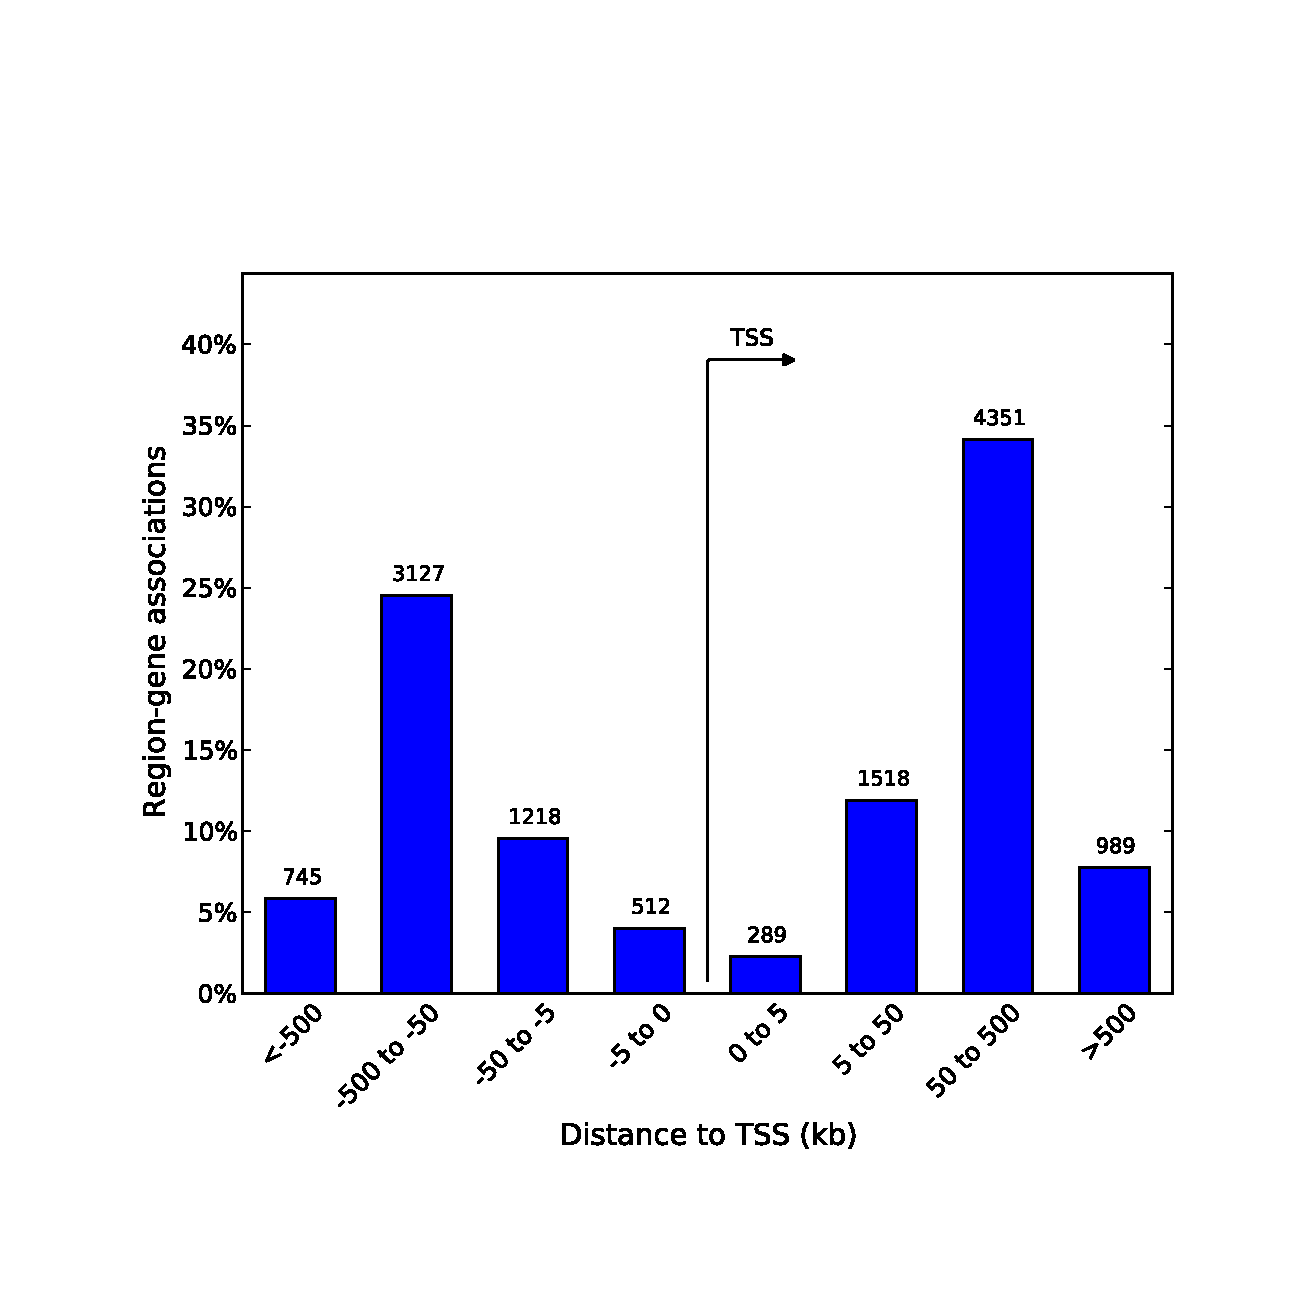
\epsfig{file=figures/autismFigureS2.pdf,width=0.8\linewidth,clip=,trim=0 0 0 0} \\
\end{tabular}
\caption[TBR1 peak distance to TSS distribution]{
{\bf TBR1 peak distance to TSS distribution.}
Distribution of TBR1 ChIP-seq peak distances to the
associated transcription start
sites.
}
\label{fig:autismFigS2}
\end{figure}

\begin{figure}[htbp]
\centering
\begin{tabular}{l}
\epsfig{file=figures/autismFigureS3.pdf,width=0.99\linewidth,clip=,trim=0 0 0 0} \\
\end{tabular}
\caption[Autism risk gene overlap between studies]{
{\bf Autism risk gene overlap between studies.}
Overlaps among the mouse orthologs of high-confidence
{\bf (A)} and probable {\bf (B)} ASD genes from different studies. \emph{SYNGAP1}
was not mapped from the high-confidence human ASD gene set to mouse.
}
\label{fig:autismFigS3}
\end{figure}

\begin{figure}[htbp]
\centering
\begin{tabular}{l}
\epsfig{file=figures/autismFigureS4.pdf,width=0.99\linewidth,clip=,trim=0 0 0 0} \\
\end{tabular}
\caption[RISH \emph{in situs} of high-confidence ASD genes]{
{\bf RISH \emph{in situs} of high-confidence ASD genes.}
Radioactive \emph{in situ} hybridization (RISH) of
high-confidence ASD genes at P0 in \emph{Tbr1}\textsuperscript{+/+} and
\emph{Tbr1\textsuperscript{-/-}} cortices reveals expression
differences.
}
\label{fig:autismFigS4}
\end{figure}

\begin{figure}[htbp]
\centering
\begin{tabular}{l}
\epsfig{file=figures/autismFigureS5.pdf,width=0.99\linewidth,clip=,trim=0 0 0 0} \\
\end{tabular}
\caption[DIG \emph{in situs} of high-confidence ASD genes]{
{\bf DIG \emph{in situs} of high-confidence ASD genes.}
Digoxigenin (DIG) \emph{in situ} hybridization of
high-confidence genes at E14.5 {\bf (A)} and P0 {\bf (B)} in
\emph{Tbr1}\textsuperscript{+/+} and \emph{Tbr1\textsuperscript{-/-}}
cortices reveals expression differences. Relative expression corresponds
to quantitative real-time PCR (qRT-PCR) results comparing transcript
expression levels in the cortex of the \emph{Tbr1} mutant mice and
wild-type littermates at E14.5 {\bf (C)} and P0 {\bf (D)}. The error bars represent
the standard error of the mean. 2-sided \emph{t}-test. **\emph{p}-value
\textless{} 0.01; ***\emph{p}-value \textless{} 0.001.
}
\label{fig:autismFigS5}
\end{figure}

\begin{figure}[htbp]
\centering
\begin{tabular}{l}
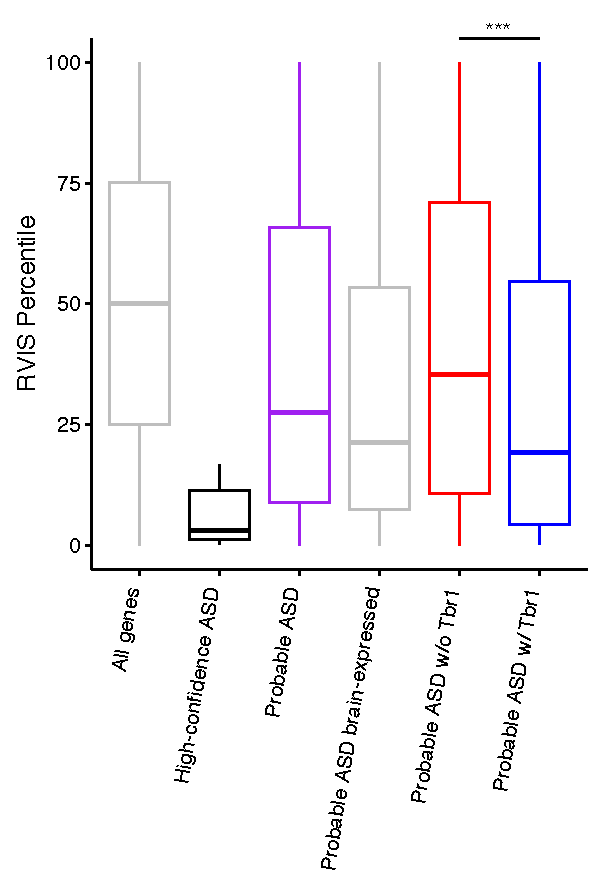
\epsfig{file=figures/autismFigureS6.pdf,width=0.6\linewidth,clip=,trim=0 0 0 0} \\
\end{tabular}
\caption[RVIS percentile distributions for ASD genes]{
{\bf RVIS percentile distributions for ASD genes.}
Probable ASD genes that are TBR1 targets are depleted
for RVIS percentiles. Box-plots depicting the distributions of RVIS
percentiles for different ASD gene lists (x-axis). Probable ASD genes
with adjacent TBR1 ChIP-seq peaks in the developing cortex (blue) have
lower RVIS percentiles than those without an adjacent TBR1 peak (red).
Significance was determined using the 1-sided 2-sample Wilcoxon test.
***\emph{p}-value \textless{} 0.001.
}
\label{fig:autismFigS6}
\end{figure}

\section{Supplemental Tables}

\begin{landscape}
\begin{center}
\begin{longtable}{@{}>{\hspace{0pt}}p{0.08\linewidth}>{\hspace{0pt}}p{0.08\linewidth}>{\hspace{0pt}}p{0.1\linewidth}>{\hspace{0pt}}p{0.17\linewidth}>{\hspace{0pt}}p{0.05\linewidth}>{\hspace{0pt}}p{0.06\linewidth}>{\hspace{0pt}}p{0.07\linewidth}>{\hspace{0pt}}p{0.05\linewidth}>{\hspace{0pt}}p{0.06\linewidth}>{\hspace{0pt}}p{0.06\linewidth}>{\hspace{0pt}}p{0.07\linewidth}@{}}
\caption[Autism risk gene metrics]{{\bf Autism risk gene metrics.}
The number of TBR1 ChIP-seq peaks adjacent to the
mouse ortholog, GREAT bionmial \emph{p-}value, fraction LoF score,
fraction LoF percentile among all genes, Icelandic knockout status, and
limma \emph{p}-value and fold for each high-confidence and probable ASD
gene. ``NA'' describes missing values.
}
\label{tab:autismTabS1} \\

\hline \textbf{Gene symbol} & \textbf{Merged gene list} & \textbf{Gene lists} & \textbf{Ensembl Identifier} & \textbf{\#
Tbr1 peaks} & \textbf{\# Tbr1 peaks GREAT binomial \emph{p}-value} & \textbf{Fraction LoF}
& \textbf{Fraction LoF percentile} & \textbf{Icelandic KO status} & \textbf{limma E14.5
log(fold-change)} & \textbf{limma E14.5 \emph{p}-value} \\ \hline 
\endfirsthead

\hline \textbf{Gene symbol} & \textbf{Merged gene list} & \textbf{Gene lists} & \textbf{Ensembl Identifier} & \textbf{\#
Tbr1 peaks} & \textbf{\# Tbr1 peaks GREAT binomial \emph{p}-value} & \textbf{Fraction LoF}
& \textbf{Fraction LoF percentile} & \textbf{Icelandic KO status} & \textbf{limma E14.5
log(fold-change)} & \textbf{limma E14.5 \emph{p}-value} \\ \hline 
\endhead

\hline
\endlastfoot

\emph{NFIB} & probable & pIossifov & ENSG00000147862 & 14 & 5.44E-05 &
3.31E-06 & 0.30 & Normal & 1.55 & 4.23E-03\tabularnewline
\emph{PBX1} & probable & pDeRubeis & ENSG00000185630 & 12 & 5.32E-03 &
1.64E-05 & 0.33 & Normal & 0.86 & 2.72E-02\tabularnewline
\emph{NFIA} & probable & pIossifov, pDeRubeis, pWillsey &
ENSG00000162599 & 12 & 4.05E-05 & 4.85E-05 & 0.41 & Normal & 1.26 &
9.09E-03\tabularnewline
\emph{ZFHX3} & probable & pIossifov & ENSG00000140836 & 12 & 6.12E-03 &
1.27E-04 & 0.54 & Normal & -0.44 & 8.92E-02\tabularnewline
\emph{MYT1L} & probable & pDeRubeis & ENSG00000186487 & 10 & 2.54E-03 &
9.87E-06 & 0.31 & Normal & 0.94 & 2.56E-02\tabularnewline
\emph{DSCAM} & high-confidence & hcIossifov, pDeRubeis & ENSG00000171587
& 10 & 3.58E-04 & 2.50E-05 & 0.36 & Normal & 0.39 &
3.29E-01\tabularnewline
\emph{INSC} & probable & pDeRubeis & ENSG00000188487 & 9 & 3.31E-03 &
3.21E-04 & 0.68 & Normal & -0.02 & 8.64E-01\tabularnewline
\emph{ELAVL2} & probable & pIossifov & ENSG00000107105 & 8 & 1.42E-01 &
3.63E-05 & 0.38 & Normal & 1.85 & 3.71E-02\tabularnewline
\emph{PARD3B} & probable & pIossifov & ENSG00000116117 & 8 & 1.06E-01 &
8.95E-05 & 0.49 & Normal & 0.17 & 2.72E-01\tabularnewline
\emph{GRIN2B} & high-confidence & hcIossifov, hcDeRubeis, hcWillsey &
ENSG00000273079 & 8 & 7.25E-03 & 1.22E-04 & 0.53 & Normal & 0.34 &
3.41E-02\tabularnewline
\emph{NBEA} & probable & pIossifov & ENSG00000172915 & 8 & 5.16E-02 &
2.67E-04 & 0.65 & Normal & 0.91 & 7.81E-02\tabularnewline
\emph{ZNF238} & probable & pDeRubeis & ENSG00000179456 & 7 & 4.99E-04 &
0.00E+00 & 0.00 & Normal & 1.17 & 2.95E-02\tabularnewline
\emph{JARID2} & probable & pDeRubeis & ENSG00000008083 & 7 & 6.36E-02 &
1.40E-05 & 0.32 & Normal & 0.21 & 4.84E-01\tabularnewline
\emph{SORCS3} & probable & pDeRubeis & ENSG00000156395 & 7 & 7.55E-02 &
5.27E-05 & 0.42 & Normal & -0.11 & 4.85E-01\tabularnewline
\emph{CMPK2} & probable & pIossifov & ENSG00000134326 & 7 & 1.47E-02 &
6.18E-05 & 0.44 & Normal & -0.11 & 6.06E-01\tabularnewline
\emph{ANK2} & high-confidence & hcIossifov, hcDeRubeis, hcWillsey &
ENSG00000145362 & 7 & 2.13E-02 & 7.41E-05 & 0.46 & Normal & 0.97 &
2.58E-02\tabularnewline
\emph{MED13L} & high-confidence & hcIossifov, pDeRubeis, pWillsey &
ENSG00000123066 & 7 & 8.64E-02 & 7.45E-05 & 0.47 & Normal & 0.60 &
4.13E-02\tabularnewline
\emph{GSDMC} & probable & pDeRubeis & ENSG00000147697 & 7 & 3.14E-02 &
8.20E-04 & 0.78 & Normal & -0.22 & 5.67E-02\tabularnewline
\emph{TBL1XR1} & probable & pIossifov & ENSG00000177565 & 6 & 5.09E-01 &
0.00E+00 & 0.00 & Normal & 0.35 & 6.64E-03\tabularnewline
\emph{CUL1} & probable & pDeRubeis & ENSG00000055130 & 6 & 1.13E-01 &
1.68E-05 & 0.33 & Normal & 0.73 & 6.35E-02\tabularnewline
\emph{RELN} & probable & pDeRubeis, pWillsey & ENSG00000189056 & 6 &
1.46E-02 & 2.12E-05 & 0.34 & Normal & 1.18 & 8.08E-03\tabularnewline
\emph{TCF4} & probable & pDeRubeis & ENSG00000196628 & 6 & 2.56E-01 &
2.42E-04 & 0.64 & Normal & 0.99 & 4.03E-03\tabularnewline
\emph{TAF4} & probable & pDeRubeis & ENSG00000130699 & 6 & 6.97E-03 &
5.95E-03 & 0.92 & Normal & -0.23 & 7.47E-02\tabularnewline
\emph{SEMA6A} & probable & pDeRubeis & ENSG00000092421 & 5 & 2.01E-01 &
5.81E-06 & 0.30 & Normal & -0.35 & 2.60E-01\tabularnewline
\emph{BAI1} & probable & pIossifov & ENSG00000181790 & 5 & 7.95E-02 &
8.34E-06 & 0.31 & Normal & 0.08 & 7.32E-01\tabularnewline
\emph{CACNA2D3} & high-confidence & hcDeRubeis, pIossifov, pWillsey &
ENSG00000157445 & 5 & 1.37E-01 & 1.18E-05 & 0.32 & Normal & -0.09 &
7.83E-01\tabularnewline
\emph{GRIA2} & probable & pDeRubeis & ENSG00000120251 & 5 & 1.74E-01 &
2.02E-05 & 0.34 & Normal & 1.12 & 1.93E-02\tabularnewline
\emph{CTNNB1} & probable & pIossifov & ENSG00000168036 & 5 & 5.39E-02 &
2.72E-05 & 0.36 & Normal & -0.28 & 4.70E-01\tabularnewline
\emph{LRP6} & probable & pIossifov & ENSG00000070018 & 5 & 6.47E-04 &
5.25E-05 & 0.42 & Normal & 0.62 & 4.11E-02\tabularnewline
\emph{ZNF462} & probable & pDeRubeis & ENSG00000148143 & 5 & 3.71E-01 &
7.64E-05 & 0.47 & Normal & 1.07 & 2.62E-02\tabularnewline
\emph{NUAK1} & probable & pIossifov, pDeRubeis, pWillsey &
ENSG00000074590 & 5 & 8.56E-02 & 8.10E-05 & 0.48 & Normal & 0.23 &
4.67E-01\tabularnewline
\emph{DNAH5} & probable & pIossifov, pDeRubeis, pWillsey &
ENSG00000039139 & 5 & 2.48E-01 & 9.37E-05 & 0.50 & Normal & -0.17 &
1.88E-01\tabularnewline
\emph{CUX2} & probable & pDeRubeis & ENSG00000111249 & 5 & 8.05E-04 &
1.28E-04 & 0.54 & Normal & -0.13 & 5.12E-01\tabularnewline
\emph{IGSF3} & probable & pIossifov & ENSG00000143061 & 5 & 2.23E-03 &
1.58E-04 & 0.57 & Normal & -0.07 & 7.98E-01\tabularnewline
\emph{NXPE4} & probable & pIossifov & ENSG00000137634 & 5 & 8.54E-02 &
2.54E-04 & 0.64 & Normal & 0.27 & 1.16E-01\tabularnewline
\emph{NFE2L3} & probable & pIossifov & ENSG00000050344 & 5 & 8.46E-02 &
3.14E-03 & 0.89 & Normal & 0.31 & 1.13E-01\tabularnewline
\emph{EPHB2} & probable & pIossifov, pDeRubeis, pWillsey &
ENSG00000133216 & 5 & 1.29E-03 & 5.43E-03 & 0.91 & Normal & -0.33 &
3.28E-02\tabularnewline
\emph{DPP4} & probable & pDeRubeis & ENSG00000197635 & 5 & 8.99E-03 &
6.73E-03 & 0.92 & Normal & -0.20 & 9.60E-02\tabularnewline
\emph{GALNT18, GALNTL4} & probable & pIossifov, pDeRubeis, pWillsey &
ENSG00000110328 & 4 & 2.78E-01 & 6.89E-06 & 0.30 & Normal & -1.00 &
2.82E-02\tabularnewline
\emph{BCL11A} & high-confidence & hcDeRubeis, pIossifov, pWillsey &
ENSG00000119866 & 4 & 4.35E-01 & 1.71E-05 & 0.33 & Normal & 1.14 &
2.61E-02\tabularnewline
\emph{CUL3} & high-confidence & hcDeRubeis, hcWillsey, pIossifov &
ENSG00000036257 & 4 & 7.10E-02 & 1.94E-05 & 0.34 & Normal & 0.81 &
7.33E-03\tabularnewline
\emph{THSD7A} & probable & pIossifov, pDeRubeis, pWillsey &
ENSG00000005108 & 4 & 4.10E-01 & 3.17E-05 & 0.37 & Normal & -0.10 &
4.66E-01\tabularnewline
\emph{LRRC4} & probable & pDeRubeis & ENSG00000128594 & 4 & 8.48E-02 &
3.24E-05 & 0.37 & Normal & -0.11 & 7.17E-01\tabularnewline
\emph{FAM190A} & probable & pDeRubeis & ENSG00000184305 & 4 & 4.71E-01 &
4.09E-05 & 0.40 & Normal & 0.45 & 3.79E-02\tabularnewline
\emph{SETBP1} & probable & pIossifov, pDeRubeis, pWillsey &
ENSG00000152217 & 4 & 5.90E-01 & 5.01E-05 & 0.42 & Normal & NA &
NA\tabularnewline
\emph{HGF} & probable & pDeRubeis & ENSG00000019991 & 4 & 6.40E-01 &
5.77E-05 & 0.43 & Normal & -0.14 & 1.68E-01\tabularnewline
\emph{WDFY3} & high-confidence & hcIossifov, pDeRubeis, pWillsey &
ENSG00000163625 & 4 & 1.49E-01 & 8.83E-05 & 0.49 & Normal & 0.24 &
7.86E-02\tabularnewline
\emph{FAM8A1} & probable & pIossifov, pDeRubeis, pWillsey &
ENSG00000137414 & 4 & 4.24E-03 & 1.10E-04 & 0.52 & Normal & 0.68 &
3.45E-01\tabularnewline
\emph{WNT7B} & probable & pIossifov & ENSG00000188064 & 4 & 2.77E-02 &
1.62E-04 & 0.58 & Normal & 0.76 & 3.40E-02\tabularnewline
\emph{CTNNA3} & probable & pIossifov & ENSG00000183230 & 4 & 1.44E-01 &
1.84E-04 & 0.60 & Normal & -0.11 & 2.31E-01\tabularnewline
\emph{DYSF} & probable & pDeRubeis & ENSG00000135636 & 4 & 1.32E-01 &
1.91E-04 & 0.60 & Normal & -0.24 & 1.28E-01\tabularnewline
\emph{GRAMD3} & probable & pDeRubeis & ENSG00000155324 & 4 & 4.02E-01 &
4.13E-04 & 0.71 & Normal & -0.24 & 6.20E-02\tabularnewline
\emph{BTBD9} & probable & pIossifov & ENSG00000183826 & 4 & 9.82E-02 &
4.43E-04 & 0.72 & Normal & 0.13 & 4.49E-01\tabularnewline
\emph{CTTNBP2} & probable & pIossifov, pDeRubeis, pWillsey &
ENSG00000077063 & 4 & 1.29E-01 & 5.77E-04 & 0.75 & Normal & 0.55 &
2.05E-01\tabularnewline
\emph{TNRC18} & probable & pIossifov & ENSG00000182095 & 4 & 3.48E-03 &
1.07E-03 & 0.81 & Normal & 0.04 & 8.09E-01\tabularnewline
\emph{NARG2} & probable & pIossifov & ENSG00000128915 & 4 & 1.95E-01 &
1.83E-03 & 0.85 & Normal & 0.08 & 3.26E-01\tabularnewline
\emph{PDE11A} & probable & pDeRubeis & ENSG00000128655 & 4 & 2.33E-02 &
2.09E-03 & 0.86 & KO & NA & NA\tabularnewline
\emph{SCN2A} & high-confidence & hcIossifov, hcDeRubeis, hcWillsey &
ENSG00000136531 & 3 & 1.45E-02 & 9.39E-06 & 0.31 & Normal & 0.27 &
2.11E-01\tabularnewline
\emph{NR3C2} & probable & pIossifov, pDeRubeis, pWillsey &
ENSG00000151623 & 3 & 8.40E-01 & 1.78E-05 & 0.33 & Normal & -0.03 &
6.93E-01\tabularnewline
\emph{SVIL} & probable & pDeRubeis & ENSG00000197321 & 3 & 3.22E-01 &
1.99E-05 & 0.34 & Normal & -0.23 & 1.33E-01\tabularnewline
\emph{WAC} & high-confidence & hcIossifov & ENSG00000095787 & 3 &
6.87E-01 & 2.05E-05 & 0.34 & Normal & 0.75 & 1.80E-01\tabularnewline
\emph{LRFN2} & probable & pIossifov & ENSG00000156564 & 3 & 5.23E-01 &
3.27E-05 & 0.37 & Normal & -0.20 & 4.88E-01\tabularnewline
\emph{FOXP1} & high-confidence & hcIossifov, pDeRubeis, pWillsey &
ENSG00000114861 & 3 & 6.83E-01 & 3.57E-05 & 0.38 & Normal & 0.47 &
1.62E-02\tabularnewline
\emph{DYRK1A} & high-confidence & hcIossifov, hcDeRubeis, hcWillsey &
ENSG00000157540 & 3 & 1.50E-01 & 3.82E-05 & 0.39 & Normal & -0.28 &
4.90E-02\tabularnewline
\emph{CSMD2} & probable & pIossifov & ENSG00000121904 & 3 & 7.71E-02 &
4.08E-05 & 0.40 & Normal & 0.13 & 6.40E-01\tabularnewline
\emph{ERBB2IP} & probable & pDeRubeis & ENSG00000112851 & 3 & 7.30E-02 &
4.67E-05 & 0.41 & Normal & 1.25 & 7.31E-02\tabularnewline
\emph{HIVEP3} & probable & pIossifov & ENSG00000127124 & 3 & 1.22E-01 &
4.83E-05 & 0.41 & Normal & 0.09 & 3.28E-01\tabularnewline
\emph{PPP1R15B} & probable & pWillsey & ENSG00000158615 & 3 & 1.90E-02 &
4.99E-05 & 0.42 & Normal & -0.28 & 2.71E-02\tabularnewline
\emph{ADAMTS9} & probable & pIossifov & ENSG00000163638 & 3 & 6.62E-01 &
5.47E-05 & 0.43 & Normal & -0.43 & 8.82E-02\tabularnewline
\emph{DSCAML1} & probable & pIossifov & ENSG00000177103 & 3 & 1.21E-01 &
5.57E-05 & 0.43 & Normal & -0.11 & 3.30E-01\tabularnewline
\emph{TUSC1} & probable & pIossifov & ENSG00000198680 & 3 & 9.25E-01 &
6.94E-05 & 0.46 & Normal & -0.16 & 5.88E-01\tabularnewline
\emph{NIN} & probable & pIossifov & ENSG00000100503 & 3 & 3.08E-02 &
9.09E-05 & 0.49 & Normal & 0.53 & 7.58E-02\tabularnewline
\emph{TRPM3} & probable & pIossifov & ENSG00000083067 & 3 & 7.45E-01 &
9.27E-05 & 0.49 & Normal & -0.30 & 5.28E-02\tabularnewline
\emph{NRXN1} & probable & pIossifov, pDeRubeis, pWillsey &
ENSG00000179915 & 3 & 9.25E-01 & 1.21E-04 & 0.53 & Normal & 1.43 &
4.38E-03\tabularnewline
\emph{SORBS1} & probable & pIossifov & ENSG00000095637 & 3 & 6.12E-02 &
1.48E-04 & 0.56 & Normal & 0.88 & 4.81E-02\tabularnewline
\emph{TTN} & probable & pDeRubeis, pDeRubeis & ENSG00000155657 & 3 &
6.69E-02 & 1.72E-04 & 0.58 & Normal & -0.10 & 4.49E-01\tabularnewline
\emph{CECR2} & probable & pDeRubeis & ENSG00000099954 & 3 & 3.01E-02 &
2.95E-04 & 0.66 & Normal & 0.22 & 2.50E-01\tabularnewline
\emph{DST} & probable & pIossifov, pDeRubeis, pWillsey & ENSG00000151914
& 3 & 1.90E-01 & 2.97E-04 & 0.67 & Normal & 0.07 &
4.14E-01\tabularnewline
\emph{RIMS1} & high-confidence & hcIossifov, pDeRubeis, pWillsey &
ENSG00000079841 & 3 & 6.10E-01 & 3.37E-04 & 0.68 & Normal & 0.17 &
3.29E-01\tabularnewline
\emph{SUCLG2} & probable & pIossifov & ENSG00000172340 & 3 & 5.38E-01 &
5.19E-04 & 0.74 & Normal & -0.40 & 3.52E-01\tabularnewline
\emph{TYW5} & probable & pIossifov & ENSG00000162971 & 3 & 8.83E-02 &
1.68E-03 & 0.84 & Normal & 0.05 & 6.49E-01\tabularnewline
\emph{KMT2E, MLL5} & high-confidence & hcIossifov, pDeRubeis, pWillsey &
ENSG00000005483 & 3 & 4.53E-01 & 9.28E-03 & 0.93 & Normal & 0.65 &
9.50E-03\tabularnewline
\emph{IRF2BPL} & probable & pIossifov & ENSG00000119669 & 3 & 2.24E-02 &
2.75E-02 & 0.96 & Normal & -0.04 & 7.48E-01\tabularnewline
\emph{SHANK2} & probable & pIossifov, pDeRubeis, pWillsey &
ENSG00000162105 & 3 & 2.79E-01 & 8.98E-02 & 0.98 & Normal & 0.34 &
1.81E-01\tabularnewline
\emph{ARMC2} & probable & pDeRubeis & ENSG00000118690 & 3 & 1.47E-01 &
3.20E-01 & 0.99 & Normal & -0.17 & 2.86E-01\tabularnewline
\emph{TBR1} & high-confidence & hcIossifov, hcDeRubeis, hcWillsey &
ENSG00000136535 & 2 & 2.43E-01 & 0.00E+00 & 0.00 & Normal & 1.29 &
1.32E-02\tabularnewline
\emph{NCKAP1} & high-confidence & hcIossifov, pDeRubeis, pWillsey &
ENSG00000061676 & 2 & 7.76E-02 & 2.64E-06 & 0.30 & Normal & 0.93 &
6.32E-02\tabularnewline
\emph{ZMYND11} & probable & pIossifov, pDeRubeis, pWillsey &
ENSG00000015171 & 2 & 8.15E-01 & 4.28E-06 & 0.30 & Normal & 0.40 &
3.15E-01\tabularnewline
\emph{RFX7} & probable & pDeRubeis & ENSG00000181827 & 2 & 1.30E-01 &
7.49E-06 & 0.31 & Normal & 1.18 & 5.21E-02\tabularnewline
\emph{ASXL3} & high-confidence & hcDeRubeis & ENSG00000141431 & 2 &
7.06E-01 & 1.80E-05 & 0.34 & Normal & 0.70 & 1.18E-02\tabularnewline
\emph{MED13} & probable & pIossifov & ENSG00000108510 & 2 & 1.29E-01 &
2.71E-05 & 0.36 & Normal & 1.46 & 5.45E-02\tabularnewline
\emph{LEO1} & probable & pDeRubeis & ENSG00000166477 & 2 & 6.51E-02 &
2.93E-05 & 0.37 & Normal & -0.24 & 5.23E-02\tabularnewline
\emph{PRPF40A} & probable & pDeRubeis & ENSG00000196504 & 2 & 2.52E-01 &
3.50E-05 & 0.38 & Normal & 0.69 & 7.19E-03\tabularnewline
\emph{SPATA13} & probable & pIossifov, pDeRubeis, pWillsey &
ENSG00000182957 & 2 & 3.01E-01 & 3.79E-05 & 0.39 & Normal & -0.19 &
4.53E-01\tabularnewline
\emph{MPP6} & probable & pIossifov & ENSG00000105926 & 2 & 3.56E-01 &
4.00E-05 & 0.39 & Normal & -0.41 & 2.63E-01\tabularnewline
\emph{TANC2} & probable & pIossifov & ENSG00000170921 & 2 & 4.01E-01 &
4.37E-05 & 0.40 & Normal & 0.91 & 3.25E-02\tabularnewline
\emph{GABRB3} & probable & pDeRubeis & ENSG00000166206 & 2 & 8.12E-01 &
6.02E-05 & 0.44 & Normal & 0.98 & 2.02E-02\tabularnewline
\emph{RIMBP2} & probable & pDeRubeis & ENSG00000060709 & 2 & 1.82E-01 &
7.63E-05 & 0.47 & Normal & NA & NA\tabularnewline
\emph{IQGAP2} & probable & pIossifov, pDeRubeis, pWillsey &
ENSG00000145703 & 2 & 3.52E-01 & 8.01E-05 & 0.48 & Normal & 0.18 &
2.91E-01\tabularnewline
\emph{CSTF2T} & probable & pIossifov, pDeRubeis, pWillsey &
ENSG00000177613 & 2 & 8.60E-01 & 9.02E-05 & 0.49 & Normal & -0.01 &
9.75E-01\tabularnewline
\emph{PRKAR1B} & probable & pDeRubeis & ENSG00000188191 & 2 & 6.58E-02 &
1.07E-04 & 0.52 & Normal & 0.31 & 4.72E-01\tabularnewline
\emph{VAV3} & probable & pIossifov & ENSG00000134215 & 2 & 7.88E-01 &
1.14E-04 & 0.52 & Normal & -0.21 & 2.07E-01\tabularnewline
\emph{CBX4} & probable & pIossifov, pDeRubeis, pWillsey &
ENSG00000141582 & 2 & 9.28E-02 & 1.93E-04 & 0.60 & Normal & 0.10 &
4.33E-01\tabularnewline
\emph{ATP10D} & probable & pIossifov, pDeRubeis, pWillsey &
ENSG00000145246 & 2 & 2.44E-01 & 1.94E-04 & 0.60 & Normal & -0.04 &
7.14E-01\tabularnewline
\emph{SPRED2} & probable & pDeRubeis & ENSG00000198369 & 2 & 8.17E-01 &
2.05E-04 & 0.61 & Normal & -0.10 & 3.29E-01\tabularnewline
\emph{ANKFN1} & probable & pIossifov & ENSG00000153930 & 2 & 4.92E-01 &
2.08E-04 & 0.61 & Normal & NA & NA\tabularnewline
\emph{XKR6} & probable & pIossifov & ENSG00000171044 & 2 & 2.19E-01 &
2.12E-04 & 0.62 & Normal & 0.35 & 3.93E-01\tabularnewline
\emph{BRCA1} & probable & pIossifov & ENSG00000012048 & 2 & 2.56E-02 &
2.51E-04 & 0.64 & Normal & -0.22 & 6.91E-02\tabularnewline
\emph{ARID1B} & high-confidence & hcIossifov, hcDeRubeis, pWillsey &
ENSG00000049618 & 2 & 9.14E-01 & 2.79E-04 & 0.66 & Normal & 0.13 &
5.25E-01\tabularnewline
\emph{PTPN13} & probable & pIossifov & ENSG00000163629 & 2 & 3.30E-01 &
4.02E-04 & 0.70 & Normal & -0.11 & 4.15E-01\tabularnewline
\emph{DNMT3A} & probable & pIossifov & ENSG00000119772 & 2 & 2.93E-01 &
4.15E-04 & 0.71 & Normal & -0.37 & 2.00E-01\tabularnewline
\emph{MTUS1} & probable & pIossifov & ENSG00000129422 & 2 & 1.99E-01 &
4.32E-04 & 0.71 & Normal & -0.13 & 2.49E-01\tabularnewline
\emph{PSD3} & probable & pIossifov & ENSG00000156011 & 2 & 6.30E-01 &
4.44E-04 & 0.72 & Normal & 0.45 & 3.88E-02\tabularnewline
\emph{RGS2} & probable & pDeRubeis & ENSG00000116741 & 2 & 3.11E-01 &
5.44E-04 & 0.74 & Normal & -0.04 & 5.97E-01\tabularnewline
\emph{LRRTM2} & probable & pDeRubeis & ENSG00000146006 & 2 & 2.94E-01 &
5.78E-04 & 0.75 & Normal & 0.37 & 2.90E-02\tabularnewline
\emph{TRIM37} & probable & pDeRubeis & ENSG00000108395 & 2 & 1.56E-01 &
6.75E-04 & 0.76 & Normal & 0.34 & 6.63E-02\tabularnewline
\emph{C10orf90} & probable & pIossifov & ENSG00000154493 & 2 & 3.54E-01
& 1.27E-03 & 0.82 & Normal & -0.12 & 3.62E-01\tabularnewline
\emph{AMBP} & probable & pIossifov & ENSG00000106927 & 2 & 1.17E-01 &
1.34E-03 & 0.83 & Normal & 0.06 & 7.43E-01\tabularnewline
\emph{EFCAB5} & probable & pIossifov, pDeRubeis, pWillsey &
ENSG00000176927 & 2 & 5.28E-02 & 2.09E-03 & 0.86 & KO & NA &
NA\tabularnewline
\emph{GPRIN1} & probable & pIossifov & ENSG00000169258 & 2 & 1.44E-02 &
1.11E-01 & 0.98 & Normal & -0.13 & 5.90E-01\tabularnewline
\emph{USP29} & probable & pIossifov & ENSG00000131864 & 2 & 1.76E-01 &
4.04E-01 & 0.99 & Normal & NA & NA\tabularnewline
\emph{3} & probable & pIossifov & ENSG00000274391 & 1 & 3.64E-01 & NA &
NA & Normal & -0.06 & 6.18E-01\tabularnewline
\emph{AHDC1} & probable & pIossifov & ENSG00000126705 & 1 & 3.50E-01 &
4.13E-06 & 0.30 & Normal & -0.17 & 1.08E-01\tabularnewline
\emph{ANKRD11} & high-confidence & hcIossifov & ENSG00000167522 & 1 &
4.54E-01 & 5.77E-06 & 0.30 & Normal & 0.31 & 5.15E-02\tabularnewline
\emph{GABRB1} & probable & pDeRubeis & ENSG00000163288 & 1 & 7.64E-01 &
6.19E-06 & 0.30 & Normal & -0.01 & 9.55E-01\tabularnewline
\emph{SMARCC2} & probable & pDeRubeis, pWillsey & ENSG00000139613 & 1 &
2.00E-01 & 7.68E-06 & 0.31 & Normal & 0.22 & 2.84E-01\tabularnewline
\emph{TRIP12} & probable & pIossifov, pDeRubeis, pWillsey &
ENSG00000153827 & 1 & 3.36E-01 & 1.03E-05 & 0.31 & Normal & 0.88 &
3.30E-02\tabularnewline
\emph{WNT9A} & probable & pIossifov & ENSG00000143816 & 1 & 2.02E-01 &
1.06E-05 & 0.31 & Normal & -0.96 & 7.24E-04\tabularnewline
\emph{FAM59A} & probable & pDeRubeis & ENSG00000141441 & 1 & 8.09E-01 &
1.71E-05 & 0.33 & Normal & 0.14 & 1.09E-01\tabularnewline
\emph{PTEN} & probable & pDeRubeis & ENSG00000171862 & 1 & 8.55E-01 &
1.84E-05 & 0.34 & Normal & 0.45 & 5.14E-03\tabularnewline
\emph{SPTBN1} & probable & pIossifov & ENSG00000115306 & 1 & 7.16E-01 &
1.95E-05 & 0.34 & Normal & 0.52 & 1.78E-02\tabularnewline
\emph{ATP1A1} & probable & pIossifov & ENSG00000163399 & 1 & 7.30E-01 &
1.95E-05 & 0.34 & Normal & -0.56 & 5.90E-02\tabularnewline
\emph{MYO1E} & probable & pIossifov & ENSG00000157483 & 1 & 5.44E-01 &
2.64E-05 & 0.36 & Normal & 0.08 & 5.42E-01\tabularnewline
\emph{HECTD1} & probable & pIossifov & ENSG00000092148 & 1 & 5.43E-01 &
2.74E-05 & 0.36 & Normal & 0.58 & 4.09E-02\tabularnewline
\emph{KAT2B} & probable & pIossifov & ENSG00000114166 & 1 & 3.38E-01 &
2.75E-05 & 0.36 & Normal & 0.45 & 4.02E-01\tabularnewline
\emph{KDM6B} & high-confidence & hcIossifov, pDeRubeis, pWillsey &
ENSG00000132510 & 1 & 3.39E-01 & 2.84E-05 & 0.36 & Normal & -0.67 &
2.13E-03\tabularnewline
\emph{IL17RA} & probable & pIossifov & ENSG00000177663 & 1 & 3.77E-01 &
2.91E-05 & 0.37 & Normal & -0.38 & 9.18E-02\tabularnewline
\emph{ILF2} & probable & pIossifov, pDeRubeis & ENSG00000143621 & 1 &
5.33E-02 & 2.93E-05 & 0.37 & Normal & 0.05 & 7.67E-01\tabularnewline
\emph{SKI} & probable & pDeRubeis & ENSG00000157933 & 1 & 3.56E-01 &
2.94E-05 & 0.37 & Normal & -0.21 & 2.74E-01\tabularnewline
\emph{UBR5} & probable & pIossifov & ENSG00000104517 & 1 & 5.09E-01 &
3.18E-05 & 0.37 & Normal & 0.20 & 6.78E-02\tabularnewline
\emph{EP300} & probable & pDeRubeis & ENSG00000100393 & 1 & 4.22E-01 &
3.33E-05 & 0.38 & Normal & 0.34 & 4.80E-02\tabularnewline
\emph{DOCK8} & probable & pDeRubeis & ENSG00000107099 & 1 & 5.32E-01 &
3.47E-05 & 0.38 & Normal & -0.16 & 8.25E-02\tabularnewline
\emph{FARP1} & probable & pIossifov, pDeRubeis, pWillsey &
ENSG00000152767 & 1 & 7.37E-01 & 3.53E-05 & 0.38 & Normal & -0.21 &
1.60E-01\tabularnewline
\emph{ARHGAP30} & probable & pIossifov & ENSG00000186517 & 1 & 9.67E-02
& 3.56E-05 & 0.38 & Normal & -0.14 & 3.13E-01\tabularnewline
\emph{AXL} & probable & pDeRubeis & ENSG00000167601 & 1 & 1.48E-01 &
3.71E-05 & 0.39 & Normal & -0.58 & 5.26E-02\tabularnewline
\emph{MYH10} & probable & pIossifov, pDeRubeis, pWillsey &
ENSG00000133026 & 1 & 5.30E-01 & 4.02E-05 & 0.39 & Normal & 0.35 &
2.29E-01\tabularnewline
\emph{NEDD9} & probable & pIossifov & ENSG00000111859 & 1 & 6.33E-01 &
4.05E-05 & 0.39 & Normal & -0.23 & 2.16E-01\tabularnewline
\emph{NF1} & probable & pIossifov & ENSG00000196712 & 1 & 5.02E-01 &
4.19E-05 & 0.40 & Normal & 0.26 & 4.27E-02\tabularnewline
\emph{KCNS3} & probable & pDeRubeis & ENSG00000170745 & 1 & 9.03E-01 &
4.26E-05 & 0.40 & Normal & 0.03 & 7.97E-01\tabularnewline
\emph{ARHGAP5} & probable & pIossifov & ENSG00000100852 & 1 & 8.18E-01 &
4.46E-05 & 0.40 & Normal & 0.03 & 8.95E-01\tabularnewline
\emph{RAPGEF4} & probable & pDeRubeis & ENSG00000091428 & 1 & 6.88E-01 &
4.92E-05 & 0.41 & Normal & -0.28 & 9.63E-02\tabularnewline
\emph{STXBP5} & probable & pDeRubeis & ENSG00000164506 & 1 & 8.77E-01 &
5.46E-05 & 0.43 & Normal & 0.12 & 2.93E-01\tabularnewline
\emph{STAM} & probable & pIossifov & ENSG00000136738 & 1 & 2.67E-01 &
5.47E-05 & 0.43 & Normal & 0.44 & 2.79E-02\tabularnewline
\emph{BAZ2B} & probable & pIossifov & ENSG00000123636 & 1 & 5.97E-01 &
5.50E-05 & 0.43 & Normal & 0.17 & 2.71E-01\tabularnewline
\emph{TTK} & probable & pDeRubeis & ENSG00000112742 & 1 & 3.16E-01 &
6.08E-05 & 0.44 & Normal & 0.12 & 6.75E-01\tabularnewline
\emph{PHF2} & high-confidence & hcIossifov, pDeRubeis, pWillsey &
ENSG00000197724 & 1 & 5.80E-01 & 6.32E-05 & 0.44 & Normal & -0.14 &
2.41E-01\tabularnewline
\emph{INTS6} & probable & pIossifov & ENSG00000102786 & 1 & 3.82E-01 &
7.42E-05 & 0.46 & Normal & NA & NA\tabularnewline
\emph{KDM5B} & high-confidence & hcIossifov, pDeRubeis & ENSG00000117139
& 1 & 2.26E-01 & 7.85E-05 & 0.47 & Normal & 0.39 &
8.64E-03\tabularnewline
\emph{SH3D19} & probable & pDeRubeis & ENSG00000109686 & 1 & 3.19E-01 &
7.91E-05 & 0.47 & Normal & -0.49 & 9.23E-03\tabularnewline
\emph{RASAL1} & probable & pDeRubeis & ENSG00000111344 & 1 & 2.34E-01 &
8.40E-05 & 0.48 & Normal & -0.05 & 6.82E-01\tabularnewline
\emph{CNOT3} & probable & pIossifov, pDeRubeis, pWillsey &
ENSG00000088038 & 1 & 8.22E-02 & 8.78E-05 & 0.49 & Normal & -0.04 &
7.89E-01\tabularnewline
\emph{CCIN} & probable & pDeRubeis & ENSG00000185972 & 1 & 1.31E-01 &
8.82E-05 & 0.49 & Normal & 0.03 & 7.10E-01\tabularnewline
\emph{OSBPL3} & probable & pDeRubeis & ENSG00000070882 & 1 & 5.75E-01 &
8.96E-05 & 0.49 & Normal & -0.27 & 2.14E-01\tabularnewline
\emph{SPARCL1} & probable & pDeRubeis & ENSG00000152583 & 1 & 2.86E-01 &
9.40E-05 & 0.50 & Normal & -0.06 & 8.76E-01\tabularnewline
\emph{OSBPL8} & probable & pIossifov & ENSG00000091039 & 1 & 5.50E-01 &
9.72E-05 & 0.50 & Normal & 1.24 & 1.20E-02\tabularnewline
\emph{CPD} & probable & pIossifov & ENSG00000108582 & 1 & 3.13E-01 &
1.09E-04 & 0.52 & Normal & 0.51 & 3.84E-02\tabularnewline
\emph{ADNP} & high-confidence & hcIossifov, hcDeRubeis, pWillsey &
ENSG00000101126 & 1 & 3.37E-01 & 1.17E-04 & 0.53 & Normal & 0.35 &
1.51E-01\tabularnewline
\emph{PCSK2} & probable & pIossifov & ENSG00000125851 & 1 & 8.94E-01 &
1.24E-04 & 0.54 & Normal & -0.16 & 5.79E-01\tabularnewline
\emph{UNC80} & probable & pIossifov, pWillsey & ENSG00000144406 & 1 &
6.56E-01 & 1.36E-04 & 0.55 & Normal & -0.01 & 9.28E-01\tabularnewline
\emph{PDCD1} & probable & pIossifov, pWillsey & ENSG00000188389 & 1 &
9.48E-01 & 1.38E-04 & 0.55 & Normal & -0.13 & 3.94E-01\tabularnewline
\emph{ZMYM2} & probable & pWillsey & ENSG00000121741 & 1 & 4.97E-01 &
1.41E-04 & 0.55 & Normal & 1.03 & 6.48E-02\tabularnewline
\emph{AMOTL1} & probable & pIossifov & ENSG00000166025 & 1 & 4.89E-01 &
1.48E-04 & 0.56 & Normal & -0.06 & 7.79E-01\tabularnewline
\emph{ACACB} & probable & pIossifov, pDeRubeis, pWillsey &
ENSG00000076555 & 1 & 3.29E-01 & 1.51E-04 & 0.56 & KO & -0.11 &
2.34E-01\tabularnewline
\emph{BTRC} & probable & pDeRubeis & ENSG00000166167 & 1 & 5.95E-01 &
1.62E-04 & 0.58 & Normal & -0.10 & 6.09E-01\tabularnewline
\emph{OLFM3} & probable & pIossifov & ENSG00000118733 & 1 & 9.91E-01 &
1.67E-04 & 0.58 & Normal & -0.09 & 3.22E-01\tabularnewline
\emph{TSPAN17} & probable & pIossifov, pDeRubeis, pWillsey &
ENSG00000048140 & 1 & 3.68E-01 & 1.83E-04 & 0.59 & Normal & -0.42 &
1.56E-01\tabularnewline
\emph{ARHGAP44} & probable & pDeRubeis & ENSG00000006740 & 1 & 5.63E-01
& 1.99E-04 & 0.61 & Normal & -0.01 & 9.77E-01\tabularnewline
\emph{TRIO} & probable & pDeRubeis & ENSG00000038382 & 1 & 7.69E-01 &
2.09E-04 & 0.62 & Normal & 0.53 & 1.01E-01\tabularnewline
\emph{CCPG1} & probable & pIossifov & ENSG00000260916 & 1 & 2.02E-01 &
2.16E-04 & 0.62 & Normal & 0.14 & 1.95E-01\tabularnewline
\emph{UTP6} & probable & pDeRubeis & ENSG00000108651 & 1 & 6.78E-01 &
2.74E-04 & 0.65 & Normal & 0.58 & 1.32E-01\tabularnewline
\emph{MAD1L1} & probable & pDeRubeis & ENSG00000002822 & 1 & 6.98E-01 &
3.70E-04 & 0.69 & Normal & -0.12 & 4.58E-01\tabularnewline
\emph{KDM4B} & probable & pDeRubeis & ENSG00000127663 & 1 & 3.86E-01 &
4.10E-04 & 0.71 & Normal & -0.04 & 8.67E-01\tabularnewline
\emph{STARD10} & probable & pIossifov & ENSG00000214530 & 1 & 9.79E-02 &
5.36E-04 & 0.74 & Normal & -0.40 & 2.17E-01\tabularnewline
\emph{C12orf51} & probable & pDeRubeis & ENSG00000173064 & 1 & 2.39E-01
& 5.42E-04 & 0.74 & Normal & 0.34 & 2.01E-01\tabularnewline
\emph{TCF7L2} & high-confidence & hcIossifov & ENSG00000148737 & 1 &
7.74E-01 & 5.62E-04 & 0.75 & Normal & -1.50 & 1.26E-01\tabularnewline
\emph{RANBP17} & probable & pDeRubeis & ENSG00000204764 & 1 & 6.53E-01 &
6.23E-04 & 0.76 & KO & -0.30 & 3.87E-02\tabularnewline
\emph{SCAMP2} & probable & pIossifov & ENSG00000140497 & 1 & 7.84E-02 &
6.64E-04 & 0.76 & Normal & -0.23 & 2.65E-01\tabularnewline
\emph{CCDC171} & probable & pIossifov & ENSG00000164989 & 1 & 9.48E-01 &
7.36E-04 & 0.77 & KO & -0.27 & 9.73E-02\tabularnewline
\emph{SRCAP} & probable & pIossifov & ENSG00000080603 & 1 & 2.40E-01 &
1.05E-03 & 0.81 & Normal & 0.33 & 9.27E-02\tabularnewline
\emph{PHF3} & probable & pIossifov & ENSG00000118482 & 1 & 9.55E-01 &
1.19E-03 & 0.82 & Normal & 0.51 & 4.30E-02\tabularnewline
\emph{INTS1} & probable & pDeRubeis & ENSG00000164880 & 1 & 1.21E-01 &
1.20E-03 & 0.82 & Normal & -0.02 & 9.08E-01\tabularnewline
\emph{C16orf13} & probable & pIossifov & ENSG00000130731 & 1 & 2.64E-02
& 1.56E-03 & 0.84 & Normal & -0.24 & 2.83E-01\tabularnewline
\emph{MYOC} & probable & pDeRubeis & ENSG00000034971 & 1 & 2.17E-01 &
2.41E-03 & 0.87 & Normal & 0.05 & 6.30E-01\tabularnewline
\emph{JAKMIP1} & probable & pIossifov & ENSG00000152969 & 1 & 5.01E-01 &
4.37E-03 & 0.90 & Normal & 0.47 & 5.38E-01\tabularnewline
\emph{KMT2C, MLL3} & high-confidence & hcDeRubeis, pIossifov, pWillsey &
ENSG00000055609 & 1 & 5.60E-01 & 6.29E-03 & 0.92 & Normal & 0.74 &
2.02E-02\tabularnewline
\emph{WDR27} & probable & pDeRubeis & ENSG00000184465 & 1 & 5.10E-01 &
7.06E-03 & 0.92 & KO & -0.01 & 9.52E-01\tabularnewline
\emph{KIF21A} & probable & pIossifov & ENSG00000139116 & 1 & 7.65E-01 &
1.89E-02 & 0.95 & Normal & 0.65 & 1.48E-01\tabularnewline
\emph{LTN1} & probable & pIossifov, pWillsey & ENSG00000198862 & 1 &
2.38E-01 & 8.04E-02 & 0.97 & KO & 0.27 & 3.14E-01\tabularnewline
\emph{GGNBP2} & probable & pDeRubeis & ENSG00000278311 & 0 & 1.00E+00 &
NA & NA & Normal & 0.71 & 4.92E-02\tabularnewline
\emph{LYPD4} & probable & pDeRubeis & ENSG00000273111 & 0 & 1.00E+00 &
NA & NA & Normal & 0.23 & 1.32E-01\tabularnewline
\emph{PPPDE1} & probable & pDeRubeis & ENSG00000268723 & 0 & 1.00E+00 &
NA & NA & Normal & 0.43 & 6.32E-02\tabularnewline
\emph{CASP8AP2} & probable & pIossifov & ENSG00000118412 & 0 & 1.00E+00
& 0.00E+00 & 0.00 & Normal & 1.24 & 3.30E-02\tabularnewline
\emph{MAP3K14} & probable & pIossifov, pDeRubeis, pWillsey &
ENSG00000006062 & 0 & 1.00E+00 & 0.00E+00 & 0.00 & Normal & -0.23 &
8.20E-02\tabularnewline
\emph{MFRP} & probable & pIossifov, pWillsey & ENSG00000259159 & 0 &
1.00E+00 & 0.00E+00 & 0.00 & Normal & -0.21 & 3.46E-01\tabularnewline
\emph{RPS6KA3} & probable & pIossifov, pDeRubeis, pWillsey &
ENSG00000177189 & 0 & 1.00E+00 & 0.00E+00 & 0.00 & Normal & 0.79 &
1.37E-01\tabularnewline
\emph{SLC38A3} & probable & pIossifov & ENSG00000188338 & 0 & 1.00E+00 &
0.00E+00 & 0.00 & Normal & -0.25 & 2.93E-01\tabularnewline
\emph{L1CAM} & probable & pIossifov, pDeRubeis, pWillsey &
ENSG00000198910 & 0 & 1.00E+00 & 1.22E-06 & 0.29 & Normal & 0.35 &
4.58E-01\tabularnewline
\emph{NMT1} & probable & pIossifov & ENSG00000136448 & 0 & 1.00E+00 &
2.43E-06 & 0.29 & Normal & -0.25 & 1.75E-01\tabularnewline
\emph{YTHDC1} & probable & pIossifov & ENSG00000083896 & 0 & 1.00E+00 &
4.67E-06 & 0.30 & Normal & 0.38 & 3.12E-01\tabularnewline
\emph{NOTCH1} & probable & pIossifov & ENSG00000148400 & 0 & 1.00E+00 &
4.83E-06 & 0.30 & Normal & 0.10 & 4.33E-01\tabularnewline
\emph{MBD5} & probable & pIossifov, pDeRubeis, pWillsey &
ENSG00000204406 & 0 & 1.00E+00 & 5.34E-06 & 0.30 & Normal & 0.50 &
6.19E-02\tabularnewline
\emph{POGZ} & high-confidence & hcIossifov, hcDeRubeis, hcWillsey &
ENSG00000143442 & 0 & 1.00E+00 & 8.27E-06 & 0.31 & Normal & -0.19 &
7.76E-02\tabularnewline
\emph{ZC3H11A} & probable & pDeRubeis & ENSG00000058673 & 0 & 1.00E+00 &
8.52E-06 & 0.31 & Normal & 0.54 & 1.34E-02\tabularnewline
\emph{ATP1B1} & probable & pIossifov, pDeRubeis, pWillsey &
ENSG00000143153 & 0 & 1.00E+00 & 8.87E-06 & 0.31 & Normal & -0.18 &
5.28E-01\tabularnewline
\emph{UBAP2L} & probable & pIossifov & ENSG00000143569 & 0 & 1.00E+00 &
9.15E-06 & 0.31 & Normal & -0.12 & 3.20E-01\tabularnewline
\emph{BTAF1} & probable & pIossifov & ENSG00000095564 & 0 & 1.00E+00 &
9.89E-06 & 0.31 & Normal & 0.50 & 3.07E-01\tabularnewline
\emph{PHF21A} & probable & pIossifov & ENSG00000135365 & 0 & 1.00E+00 &
1.11E-05 & 0.31 & Normal & 0.62 & 7.26E-02\tabularnewline
\emph{APBB1} & probable & pIossifov & ENSG00000166313 & 0 & 1.00E+00 &
1.23E-05 & 0.32 & Normal & -0.09 & 7.70E-01\tabularnewline
\emph{CHD1} & probable & pIossifov & ENSG00000153922 & 0 & 1.00E+00 &
1.38E-05 & 0.32 & Normal & 0.49 & 1.09E-01\tabularnewline
\emph{PLEKHO1} & probable & pIossifov & ENSG00000023902 & 0 & 1.00E+00 &
1.52E-05 & 0.33 & Normal & -0.20 & 3.56E-01\tabularnewline
\emph{DIP2A} & high-confidence & hcIossifov, pDeRubeis, pWillsey &
ENSG00000160305 & 0 & 1.00E+00 & 1.65E-05 & 0.33 & Normal & -0.38 &
3.07E-02\tabularnewline
\emph{RAB2A} & probable & pIossifov, pDeRubeis, pWillsey &
ENSG00000104388 & 0 & 1.00E+00 & 1.71E-05 & 0.33 & Normal & -0.14 &
2.25E-01\tabularnewline
\emph{KMT2A, MLL} & probable & pIossifov, pDeRubeis & ENSG00000118058 &
0 & 1.00E+00 & 1.72E-05 & 0.33 & Normal & 0.52 & 6.67E-02\tabularnewline
\emph{PSMD12} & probable & pIossifov & ENSG00000197170 & 0 & 1.00E+00 &
1.73E-05 & 0.33 & Normal & -0.13 & 5.90E-01\tabularnewline
\emph{PTMS} & probable & pDeRubeis & ENSG00000159335 & 0 & 1.00E+00 &
1.74E-05 & 0.33 & Normal & 0.10 & 6.68E-01\tabularnewline
\emph{C11orf30} & probable & pDeRubeis & ENSG00000158636 & 0 & 1.00E+00
& 1.83E-05 & 0.34 & Normal & 0.51 & 2.75E-02\tabularnewline
\emph{UNC79} & probable & pIossifov & ENSG00000133958 & 0 & 1.00E+00 &
1.88E-05 & 0.34 & Normal & NA & NA\tabularnewline
\emph{CDC73} & probable & pDeRubeis & ENSG00000134371 & 0 & 1.00E+00 &
1.94E-05 & 0.34 & Normal & 0.18 & 7.85E-02\tabularnewline
\emph{MORC3} & probable & pIossifov & ENSG00000159256 & 0 & 1.00E+00 &
2.02E-05 & 0.34 & Normal & 0.93 & 2.42E-02\tabularnewline
\emph{GOPC} & probable & pIossifov & ENSG00000047932 & 0 & 1.00E+00 &
2.05E-05 & 0.34 & Normal & 0.27 & 3.30E-02\tabularnewline
\emph{CDC42BPB} & probable & pIossifov, pDeRubeis, pWillsey &
ENSG00000198752 & 0 & 1.00E+00 & 2.08E-05 & 0.34 & Normal & -0.01 &
9.30E-01\tabularnewline
\emph{NACC1} & probable & pIossifov & ENSG00000160877 & 0 & 1.00E+00 &
2.15E-05 & 0.35 & Normal & -0.06 & 5.82E-01\tabularnewline
\emph{TNFRSF8} & probable & pIossifov & ENSG00000120949 & 0 & 1.00E+00 &
2.20E-05 & 0.35 & Normal & -0.15 & 2.18E-01\tabularnewline
\emph{SMURF1} & probable & pDeRubeis & ENSG00000198742 & 0 & 1.00E+00 &
2.24E-05 & 0.35 & Normal & -0.23 & 1.91E-01\tabularnewline
\emph{ZC3H4} & probable & pIossifov & ENSG00000130749 & 0 & 1.00E+00 &
2.46E-05 & 0.35 & Normal & -0.02 & 8.39E-01\tabularnewline
\emph{DIP2C} & probable & pIossifov, pDeRubeis, pWillsey &
ENSG00000151240 & 0 & 1.00E+00 & 2.68E-05 & 0.36 & Normal & 0.29 &
4.21E-01\tabularnewline
\emph{GOLGA5} & probable & pIossifov & ENSG00000066455 & 0 & 1.00E+00 &
2.68E-05 & 0.36 & Normal & 0.13 & 5.83E-01\tabularnewline
\emph{NOL6} & probable & pDeRubeis & ENSG00000165271 & 0 & 1.00E+00 &
2.83E-05 & 0.36 & Normal & -0.05 & 7.10E-01\tabularnewline
\emph{ITGA5} & probable & pDeRubeis, pWillsey & ENSG00000161638 & 0 &
1.00E+00 & 2.96E-05 & 0.37 & Normal & -0.70 & 7.64E-02\tabularnewline
\emph{ASH1L} & high-confidence & hcDeRubeis, pIossifov, pWillsey &
ENSG00000116539 & 0 & 1.00E+00 & 2.99E-05 & 0.37 & Normal & 0.93 &
1.19E-02\tabularnewline
\emph{JUP} & probable & pDeRubeis & ENSG00000173801 & 0 & 1.00E+00 &
3.00E-05 & 0.37 & Normal & -0.19 & 4.82E-01\tabularnewline
\emph{SETD2} & probable & pIossifov, pDeRubeis, pWillsey &
ENSG00000181555 & 0 & 1.00E+00 & 3.00E-05 & 0.37 & Normal & 0.34 &
2.46E-02\tabularnewline
\emph{DLL1} & probable & pIossifov, pDeRubeis, pWillsey &
ENSG00000198719 & 0 & 1.00E+00 & 3.12E-05 & 0.37 & Normal & -0.16 &
3.29E-01\tabularnewline
\emph{RPL12} & probable & pDeRubeis & ENSG00000197958 & 0 & 1.00E+00 &
3.70E-05 & 0.39 & Normal & -0.22 & 1.62E-01\tabularnewline
\emph{CSDE1} & probable & pIossifov, pDeRubeis, pWillsey &
ENSG00000009307 & 0 & 1.00E+00 & 3.71E-05 & 0.39 & Normal & 0.79 &
8.39E-02\tabularnewline
\emph{TNRC6B} & high-confidence & hcIossifov & ENSG00000100354 & 0 &
1.00E+00 & 3.81E-05 & 0.39 & Normal & 0.52 & 6.71E-02\tabularnewline
\emph{KLHDC10} & probable & pIossifov & ENSG00000128607 & 0 & 1.00E+00 &
3.95E-05 & 0.39 & Normal & -0.32 & 1.07E-01\tabularnewline
\emph{MUC5B} & probable & pIossifov & ENSG00000117983 & 0 & 1.00E+00 &
4.03E-05 & 0.39 & Normal & -0.02 & 8.81E-01\tabularnewline
\emph{UBR3} & probable & pIossifov, pDeRubeis, pWillsey &
ENSG00000144357 & 0 & 1.00E+00 & 4.32E-05 & 0.40 & Normal & 0.31 &
1.63E-01\tabularnewline
\emph{KDM1B} & probable & pDeRubeis & ENSG00000165097 & 0 & 1.00E+00 &
4.32E-05 & 0.40 & Normal & 0.15 & 5.06E-01\tabularnewline
\emph{COL5A3} & probable & pIossifov & ENSG00000080573 & 0 & 1.00E+00 &
4.46E-05 & 0.40 & Normal & -0.16 & 1.73E-01\tabularnewline
\emph{MDN1} & probable & pIossifov & ENSG00000112159 & 0 & 1.00E+00 &
4.47E-05 & 0.40 & Normal & 0.20 & 1.65E-01\tabularnewline
\emph{REXO1} & probable & pIossifov & ENSG00000079313 & 0 & 1.00E+00 &
4.65E-05 & 0.41 & Normal & -0.12 & 5.17E-01\tabularnewline
\emph{PHF15} & probable & pDeRubeis & ENSG00000043143 & 0 & 1.00E+00 &
5.00E-05 & 0.42 & Normal & -0.28 & 9.35E-02\tabularnewline
\emph{UGT1A6} & probable & pIossifov & ENSG00000167165 & 0 & 1.00E+00 &
5.01E-05 & 0.42 & Normal & -0.70 & 6.25E-02\tabularnewline
\emph{OVOL1} & probable & pDeRubeis & ENSG00000172818 & 0 & 1.00E+00 &
5.19E-05 & 0.42 & Normal & -0.29 & 9.74E-02\tabularnewline
\emph{FAM91A1} & probable & pIossifov, pDeRubeis, pWillsey &
ENSG00000176853 & 0 & 1.00E+00 & 5.54E-05 & 0.43 & Normal & 0.20 &
4.58E-01\tabularnewline
\emph{MOV10} & probable & pIossifov & ENSG00000155363 & 0 & 1.00E+00 &
5.55E-05 & 0.43 & Normal & -0.30 & 1.04E-01\tabularnewline
\emph{DENND5A} & probable & pDeRubeis & ENSG00000184014 & 0 & 1.00E+00 &
5.57E-05 & 0.43 & Normal & 0.33 & 1.10E-01\tabularnewline
\emph{BIRC3} & probable & pDeRubeis & ENSG00000023445 & 0 & 1.00E+00 &
5.61E-05 & 0.43 & Normal & -0.15 & 1.44E-01\tabularnewline
\emph{CTCF} & probable & pIossifov & ENSG00000102974 & 0 & 1.00E+00 &
5.71E-05 & 0.43 & Normal & 0.39 & 8.20E-02\tabularnewline
\emph{B4GALNT1} & probable & pIossifov & ENSG00000135454 & 0 & 1.00E+00
& 5.86E-05 & 0.43 & Normal & 0.00 & 9.99E-01\tabularnewline
\emph{BRWD1} & probable & pIossifov, pDeRubeis, pWillsey &
ENSG00000185658 & 0 & 1.00E+00 & 5.88E-05 & 0.44 & Normal & 1.11 &
4.09E-02\tabularnewline
\emph{UGT1A9} & probable & pIossifov & ENSG00000241119 & 0 & 1.00E+00 &
5.97E-05 & 0.44 & Normal & -0.70 & 6.25E-02\tabularnewline
\emph{PAFAH1B2} & probable & pIossifov & ENSG00000168092 & 0 & 1.00E+00
& 6.05E-05 & 0.44 & Normal & 0.41 & 1.66E-01\tabularnewline
\emph{PHF7} & probable & pIossifov, pDeRubeis, pWillsey &
ENSG00000010318 & 0 & 1.00E+00 & 6.06E-05 & 0.44 & Normal & 0.07 &
4.57E-01\tabularnewline
\emph{ADCY9} & probable & pIossifov & ENSG00000162104 & 0 & 1.00E+00 &
6.06E-05 & 0.44 & Normal & 0.07 & 6.39E-01\tabularnewline
\emph{SPAST} & probable & pIossifov, pDeRubeis, pWillsey &
ENSG00000021574 & 0 & 1.00E+00 & 6.28E-05 & 0.44 & Normal & 0.93 &
1.49E-01\tabularnewline
\emph{DOCK5} & probable & pIossifov & ENSG00000147459 & 0 & 1.00E+00 &
6.49E-05 & 0.45 & Normal & -0.16 & 1.45E-01\tabularnewline
\emph{MGRN1} & probable & pDeRubeis & ENSG00000102858 & 0 & 1.00E+00 &
6.58E-05 & 0.45 & Normal & -0.23 & 1.32E-01\tabularnewline
\emph{PLXNB1} & probable & pDeRubeis, pWillsey & ENSG00000164050 & 0 &
1.00E+00 & 6.69E-05 & 0.45 & Normal & -0.03 & 7.44E-01\tabularnewline
\emph{FAM169A} & probable & pDeRubeis & ENSG00000198780 & 0 & 1.00E+00 &
6.79E-05 & 0.45 & Normal & 0.16 & 9.59E-02\tabularnewline
\emph{FAM40A} & probable & pDeRubeis & ENSG00000143093 & 0 & 1.00E+00 &
7.01E-05 & 0.46 & Normal & -0.05 & 7.62E-01\tabularnewline
\emph{COL25A1} & probable & pIossifov, pDeRubeis, pWillsey &
ENSG00000188517 & 0 & 1.00E+00 & 7.01E-05 & 0.46 & Normal & -0.18 &
1.48E-01\tabularnewline
\emph{KDM3A} & probable & pDeRubeis & ENSG00000115548 & 0 & 1.00E+00 &
7.10E-05 & 0.46 & Normal & 0.70 & 2.98E-01\tabularnewline
\emph{SIK3} & probable & pIossifov & ENSG00000160584 & 0 & 1.00E+00 &
7.64E-05 & 0.47 & Normal & -0.20 & 1.29E-01\tabularnewline
\emph{PLVAP} & probable & pDeRubeis & ENSG00000130300 & 0 & 1.00E+00 &
7.74E-05 & 0.47 & Normal & -0.63 & 4.29E-02\tabularnewline
\emph{C20orf194} & probable & pDeRubeis & ENSG00000088854 & 0 & 1.00E+00
& 7.91E-05 & 0.47 & Normal & 0.70 & 2.99E-02\tabularnewline
\emph{SETD5} & probable & pDeRubeis & ENSG00000168137 & 0 & 1.00E+00 &
8.20E-05 & 0.48 & Normal & 0.38 & 7.25E-02\tabularnewline
\emph{RCBTB1} & probable & pIossifov & ENSG00000136144 & 0 & 1.00E+00 &
8.52E-05 & 0.48 & Normal & 0.14 & 5.33E-01\tabularnewline
\emph{SRPK2} & probable & pDeRubeis & ENSG00000135250 & 0 & 1.00E+00 &
8.81E-05 & 0.49 & Normal & 0.42 & 5.11E-02\tabularnewline
\emph{BIRC6} & probable & pDeRubeis & ENSG00000115760 & 0 & 1.00E+00 &
8.88E-05 & 0.49 & Normal & 0.25 & 6.74E-02\tabularnewline
\emph{RANBP2} & probable & pIossifov & ENSG00000153201 & 0 & 1.00E+00 &
8.96E-05 & 0.49 & Normal & 0.19 & 6.29E-01\tabularnewline
\emph{PAX5} & probable & pIossifov, pDeRubeis, pWillsey &
ENSG00000196092 & 0 & 1.00E+00 & 9.11E-05 & 0.49 & Normal & -0.14 &
1.33E-01\tabularnewline
\emph{LARP4B} & probable & pIossifov & ENSG00000107929 & 0 & 1.00E+00 &
9.18E-05 & 0.49 & Normal & 0.81 & 9.24E-02\tabularnewline
\emph{ZC3H14} & probable & pDeRubeis & ENSG00000100722 & 0 & 1.00E+00 &
9.21E-05 & 0.49 & Normal & -0.30 & 1.05E-01\tabularnewline
\emph{PCDHA13} & probable & pIossifov & ENSG00000239389 & 0 & 1.00E+00 &
9.24E-05 & 0.49 & Normal & 0.60 & 1.21E-01\tabularnewline
\emph{UGT1A7} & probable & pIossifov & ENSG00000244122 & 0 & 1.00E+00 &
9.30E-05 & 0.50 & Normal & -0.70 & 6.25E-02\tabularnewline
\emph{MSH4} & probable & pDeRubeis & ENSG00000057468 & 0 & 1.00E+00 &
9.40E-05 & 0.50 & Normal & 0.12 & 2.24E-01\tabularnewline
\emph{IL27} & probable & pDeRubeis & ENSG00000197272 & 0 & 1.00E+00 &
9.49E-05 & 0.50 & Normal & NA & NA\tabularnewline
\emph{PINK1} & probable & pIossifov & ENSG00000158828 & 0 & 1.00E+00 &
9.52E-05 & 0.50 & Normal & -0.07 & 8.44E-01\tabularnewline
\emph{TLK2} & probable & pIossifov & ENSG00000146872 & 0 & 1.00E+00 &
9.55E-05 & 0.50 & Normal & 0.47 & 3.54E-02\tabularnewline
\emph{TSPAN4} & probable & pIossifov & ENSG00000214063 & 0 & 1.00E+00 &
9.68E-05 & 0.50 & Normal & -0.68 & 2.33E-02\tabularnewline
\emph{SLC7A7} & probable & pIossifov, pDeRubeis, pWillsey &
ENSG00000155465 & 0 & 1.00E+00 & 9.82E-05 & 0.50 & Normal & -0.32 &
7.54E-02\tabularnewline
\emph{GIGYF2} & probable & pIossifov & ENSG00000204120 & 0 & 1.00E+00 &
9.90E-05 & 0.50 & Normal & 0.31 & 7.74E-02\tabularnewline
\emph{EIF2AK2} & probable & pIossifov & ENSG00000055332 & 0 & 1.00E+00 &
1.02E-04 & 0.51 & Normal & -0.08 & 4.32E-01\tabularnewline
\emph{ARVCF} & probable & pIossifov & ENSG00000099889 & 0 & 1.00E+00 &
1.04E-04 & 0.51 & Normal & -0.18 & 1.43E-01\tabularnewline
\emph{PTPRR} & probable & pDeRubeis & ENSG00000153233 & 0 & 1.00E+00 &
1.10E-04 & 0.52 & Normal & -0.04 & 8.11E-01\tabularnewline
\emph{DPP3} & probable & pDeRubeis & ENSG00000254986 & 0 & 1.00E+00 &
1.14E-04 & 0.52 & Normal & -0.18 & 3.07E-01\tabularnewline
\emph{ZWILCH} & probable & pIossifov & ENSG00000174442 & 0 & 1.00E+00 &
1.17E-04 & 0.53 & Normal & 0.26 & 7.15E-01\tabularnewline
\emph{BTN1A1} & probable & pIossifov, pDeRubeis, pWillsey &
ENSG00000124557 & 0 & 1.00E+00 & 1.17E-04 & 0.53 & Normal & 0.09 &
3.09E-01\tabularnewline
\emph{UGT1A10} & probable & pIossifov & ENSG00000242515 & 0 & 1.00E+00 &
1.20E-04 & 0.53 & Normal & -0.70 & 6.25E-02\tabularnewline
\emph{SLC25A39} & probable & pIossifov, pDeRubeis, pWillsey &
ENSG00000013306 & 0 & 1.00E+00 & 1.20E-04 & 0.53 & Normal & -0.24 &
2.52E-01\tabularnewline
\emph{FRYL} & probable & pDeRubeis & ENSG00000075539 & 0 & 1.00E+00 &
1.20E-04 & 0.53 & Normal & 0.81 & 2.34E-02\tabularnewline
\emph{LRRFIP1} & probable & pIossifov & ENSG00000124831 & 0 & 1.00E+00 &
1.21E-04 & 0.53 & Normal & -0.13 & 3.55E-01\tabularnewline
\emph{DGKD} & probable & pDeRubeis & ENSG00000077044 & 0 & 1.00E+00 &
1.23E-04 & 0.53 & Normal & 0.18 & 9.59E-02\tabularnewline
\emph{TROVE2} & probable & pIossifov, pDeRubeis, pWillsey &
ENSG00000116747 & 0 & 1.00E+00 & 1.26E-04 & 0.54 & Normal & 0.73 &
2.33E-02\tabularnewline
\emph{NFKBIL1} & probable & pIossifov, pDeRubeis, pWillsey &
ENSG00000204498 & 0 & 1.00E+00 & 1.28E-04 & 0.54 & Normal & -0.38 &
1.92E-01\tabularnewline
\emph{PCYT1A} & probable & pDeRubeis, pWillsey & ENSG00000161217 & 0 &
1.00E+00 & 1.28E-04 & 0.54 & Normal & 0.24 & 1.02E-01\tabularnewline
\emph{TECTA} & probable & pIossifov & ENSG00000109927 & 0 & 1.00E+00 &
1.29E-04 & 0.54 & Normal & -0.13 & 2.80E-01\tabularnewline
\emph{BST2} & probable & pIossifov & ENSG00000130303 & 0 & 1.00E+00 &
1.30E-04 & 0.54 & Normal & -0.13 & 3.99E-01\tabularnewline
\emph{LDB1} & probable & pDeRubeis & ENSG00000198728 & 0 & 1.00E+00 &
1.30E-04 & 0.54 & Normal & 0.01 & 9.59E-01\tabularnewline
\emph{DBX2} & probable & pDeRubeis & ENSG00000185610 & 0 & 1.00E+00 &
1.31E-04 & 0.54 & Normal & -0.04 & 6.48E-01\tabularnewline
\emph{MPHOSPH8} & probable & pIossifov, pDeRubeis, pWillsey &
ENSG00000196199 & 0 & 1.00E+00 & 1.33E-04 & 0.55 & Normal & 0.22 &
2.69E-01\tabularnewline
\emph{MYO9B} & probable & pDeRubeis & ENSG00000099331 & 0 & 1.00E+00 &
1.36E-04 & 0.55 & Normal & 0.05 & 5.87E-01\tabularnewline
\emph{SIX2} & probable & pDeRubeis & ENSG00000170577 & 0 & 1.00E+00 &
1.37E-04 & 0.55 & Normal & -1.02 & 2.31E-02\tabularnewline
\emph{CDAN1} & probable & pIossifov & ENSG00000140326 & 0 & 1.00E+00 &
1.40E-04 & 0.55 & Normal & -0.20 & 1.46E-01\tabularnewline
\emph{BRSK2} & probable & pDeRubeis & ENSG00000174672 & 0 & 1.00E+00 &
1.43E-04 & 0.56 & Normal & 0.22 & 4.39E-01\tabularnewline
\emph{SH2B1} & probable & pIossifov & ENSG00000178188 & 0 & 1.00E+00 &
1.45E-04 & 0.56 & Normal & -0.03 & 7.30E-01\tabularnewline
\emph{RPAP1} & probable & pIossifov & ENSG00000103932 & 0 & 1.00E+00 &
1.45E-04 & 0.56 & Normal & -0.25 & 1.37E-01\tabularnewline
\emph{FAM168B} & probable & pIossifov & ENSG00000152102 & 0 & 1.00E+00 &
1.46E-04 & 0.56 & Normal & 0.06 & 7.52E-01\tabularnewline
\emph{HEATR5B} & probable & pDeRubeis & ENSG00000008869 & 0 & 1.00E+00 &
1.47E-04 & 0.56 & Normal & -0.10 & 4.28E-01\tabularnewline
\emph{FPGS} & probable & pDeRubeis & ENSG00000136877 & 0 & 1.00E+00 &
1.47E-04 & 0.56 & Normal & -0.16 & 3.56E-01\tabularnewline
\emph{POLRMT} & probable & pIossifov, pDeRubeis, pWillsey &
ENSG00000099821 & 0 & 1.00E+00 & 1.48E-04 & 0.56 & Normal & 0.08 &
5.95E-01\tabularnewline
\emph{UGT1A4} & probable & pIossifov & ENSG00000244474 & 0 & 1.00E+00 &
1.48E-04 & 0.56 & Normal & -0.70 & 6.25E-02\tabularnewline
\emph{MYH2} & probable & pIossifov & ENSG00000125414 & 0 & 1.00E+00 &
1.49E-04 & 0.56 & Normal & -0.11 & 1.96E-01\tabularnewline
\emph{PRSS38} & probable & pIossifov & ENSG00000185888 & 0 & 1.00E+00 &
1.53E-04 & 0.57 & Normal & NA & NA\tabularnewline
\emph{HSPA13} & probable & pDeRubeis & ENSG00000155304 & 0 & 1.00E+00 &
1.54E-04 & 0.57 & Normal & 0.48 & 6.56E-03\tabularnewline
\emph{URB1} & probable & pIossifov & ENSG00000142207 & 0 & 1.00E+00 &
1.54E-04 & 0.57 & Normal & 0.17 & 2.47E-01\tabularnewline
\emph{TBC1D23} & probable & pIossifov, pDeRubeis, pWillsey &
ENSG00000036054 & 0 & 1.00E+00 & 1.54E-04 & 0.57 & Normal & 0.13 &
5.31E-01\tabularnewline
\emph{LRP2} & probable & pIossifov & ENSG00000081479 & 0 & 1.00E+00 &
1.59E-04 & 0.57 & Normal & -0.15 & 2.64E-01\tabularnewline
\emph{IFT88} & probable & pIossifov & ENSG00000032742 & 0 & 1.00E+00 &
1.60E-04 & 0.57 & Normal & 0.01 & 9.35E-01\tabularnewline
\emph{CUBN} & probable & pIossifov, pDeRubeis, pWillsey &
ENSG00000107611 & 0 & 1.00E+00 & 1.60E-04 & 0.57 & Normal & 0.05 &
6.03E-01\tabularnewline
\emph{SUFU} & probable & pIossifov & ENSG00000107882 & 0 & 1.00E+00 &
1.60E-04 & 0.57 & Normal & -0.16 & 1.85E-01\tabularnewline
\emph{QRICH1} & probable & pDeRubeis & ENSG00000198218 & 0 & 1.00E+00 &
1.63E-04 & 0.58 & Normal & 0.03 & 7.86E-01\tabularnewline
\emph{DHX57} & probable & pDeRubeis & ENSG00000163214 & 0 & 1.00E+00 &
1.64E-04 & 0.58 & KO & 0.33 & 2.54E-01\tabularnewline
\emph{SKIDA1} & probable & pIossifov & ENSG00000180592 & 0 & 1.00E+00 &
1.65E-04 & 0.58 & Normal & 0.03 & 7.60E-01\tabularnewline
\emph{RNF213} & probable & pIossifov & ENSG00000173821 & 0 & 1.00E+00 &
1.65E-04 & 0.58 & KO & -0.12 & 2.73E-01\tabularnewline
\emph{FBXO11} & probable & pIossifov & ENSG00000138081 & 0 & 1.00E+00 &
1.67E-04 & 0.58 & Normal & 0.56 & 2.06E-01\tabularnewline
\emph{TRPM5} & probable & pIossifov, pDeRubeis, pWillsey &
ENSG00000070985 & 0 & 1.00E+00 & 1.69E-04 & 0.58 & Normal & -0.18 &
5.61E-02\tabularnewline
\emph{NDST4} & probable & pIossifov & ENSG00000138653 & 0 & 1.00E+00 &
1.73E-04 & 0.59 & Normal & -0.06 & 6.65E-01\tabularnewline
\emph{CHD2} & high-confidence & hcIossifov & ENSG00000173575 & 0 &
1.00E+00 & 1.76E-04 & 0.59 & Normal & 0.33 & 1.97E-01\tabularnewline
\emph{DOT1L} & probable & pIossifov & ENSG00000104885 & 0 & 1.00E+00 &
1.86E-04 & 0.60 & Normal & 0.08 & 4.02E-01\tabularnewline
\emph{NAPRT1} & probable & pIossifov, pDeRubeis, pWillsey &
ENSG00000147813 & 0 & 1.00E+00 & 1.87E-04 & 0.60 & Normal & -0.28 &
1.51E-01\tabularnewline
\emph{SPP2} & probable & pDeRubeis, pWillsey & ENSG00000072080 & 0 &
1.00E+00 & 1.97E-04 & 0.61 & Normal & 0.01 & 9.23E-01\tabularnewline
\emph{MTHFS} & probable & pDeRubeis, pWillsey & ENSG00000136371 & 0 &
1.00E+00 & 1.97E-04 & 0.61 & Normal & -0.31 & 9.80E-02\tabularnewline
\emph{RAD21L1} & probable & pIossifov, pDeRubeis, pWillsey &
ENSG00000244588 & 0 & 1.00E+00 & 2.00E-04 & 0.61 & Normal & NA &
NA\tabularnewline
\emph{ZNF292} & probable & pDeRubeis & ENSG00000188994 & 0 & 1.00E+00 &
2.01E-04 & 0.61 & Normal & 0.92 & 3.85E-02\tabularnewline
\emph{SUV420H1} & high-confidence & hcDeRubeis, pIossifov, pWillsey &
ENSG00000110066 & 0 & 1.00E+00 & 2.05E-04 & 0.61 & Normal & 0.35 &
7.16E-02\tabularnewline
\emph{C11orf24} & probable & pIossifov & ENSG00000171067 & 0 & 1.00E+00
& 2.07E-04 & 0.61 & Normal & -0.12 & 5.15E-01\tabularnewline
\emph{ST3GAL6} & probable & pDeRubeis & ENSG00000064225 & 0 & 1.00E+00 &
2.08E-04 & 0.61 & Normal & -0.12 & 2.06E-01\tabularnewline
\emph{ECE1} & probable & pIossifov & ENSG00000117298 & 0 & 1.00E+00 &
2.10E-04 & 0.62 & Normal & -0.34 & 7.19E-02\tabularnewline
\emph{LIG3} & probable & pIossifov & ENSG00000005156 & 0 & 1.00E+00 &
2.10E-04 & 0.62 & Normal & -0.32 & 3.21E-02\tabularnewline
\emph{ADSS} & probable & pDeRubeis & ENSG00000035687 & 0 & 1.00E+00 &
2.15E-04 & 0.62 & Normal & 0.13 & 7.84E-01\tabularnewline
\emph{MAK} & probable & pDeRubeis & ENSG00000111837 & 0 & 1.00E+00 &
2.18E-04 & 0.62 & Normal & -0.08 & 6.33E-01\tabularnewline
\emph{RNF38} & probable & pIossifov, pDeRubeis, pWillsey &
ENSG00000137075 & 0 & 1.00E+00 & 2.20E-04 & 0.62 & Normal & -0.38 &
1.13E-02\tabularnewline
\emph{MTMR12} & probable & pDeRubeis, pWillsey & ENSG00000150712 & 0 &
1.00E+00 & 2.24E-04 & 0.62 & Normal & -0.13 & 5.66E-01\tabularnewline
\emph{UBN2} & probable & pIossifov, pDeRubeis, pWillsey &
ENSG00000157741 & 0 & 1.00E+00 & 2.28E-04 & 0.63 & Normal & 0.58 &
7.33E-02\tabularnewline
\emph{PLA1A} & probable & pDeRubeis & ENSG00000144837 & 0 & 1.00E+00 &
2.31E-04 & 0.63 & Normal & -0.22 & 1.55E-01\tabularnewline
\emph{AKAP9} & probable & pIossifov & ENSG00000127914 & 0 & 1.00E+00 &
2.37E-04 & 0.63 & Normal & 1.21 & 5.61E-02\tabularnewline
\emph{KLB} & probable & pIossifov & ENSG00000134962 & 0 & 1.00E+00 &
2.42E-04 & 0.64 & Normal & -0.03 & 7.79E-01\tabularnewline
\emph{KIAA1731} & probable & pIossifov & ENSG00000166004 & 0 & 1.00E+00
& 2.46E-04 & 0.64 & Normal & 0.57 & 1.58E-01\tabularnewline
\emph{ASB4} & probable & pDeRubeis & ENSG00000005981 & 0 & 1.00E+00 &
2.49E-04 & 0.64 & KO & -0.17 & 4.42E-01\tabularnewline
\emph{SMAP2} & probable & pIossifov & ENSG00000084070 & 0 & 1.00E+00 &
2.56E-04 & 0.64 & Normal & 0.01 & 9.81E-01\tabularnewline
\emph{RUNDC1} & probable & pIossifov & ENSG00000198863 & 0 & 1.00E+00 &
2.58E-04 & 0.64 & Normal & -0.09 & 5.47E-01\tabularnewline
\emph{NRG4} & probable & pDeRubeis & ENSG00000169752 & 0 & 1.00E+00 &
2.61E-04 & 0.65 & Normal & -0.13 & 3.42E-01\tabularnewline
\emph{TUBGCP4} & probable & pDeRubeis, pWillsey & ENSG00000137822 & 0 &
1.00E+00 & 2.67E-04 & 0.65 & Normal & 0.50 & 2.45E-02\tabularnewline
\emph{GIGYF1} & high-confidence & hcIossifov & ENSG00000146830 & 0 &
1.00E+00 & 2.68E-04 & 0.65 & Normal & 0.09 & 4.81E-01\tabularnewline
\emph{SCUBE2} & probable & pIossifov, pDeRubeis, pWillsey &
ENSG00000175356 & 0 & 1.00E+00 & 2.70E-04 & 0.65 & Normal & -0.15 &
2.46E-01\tabularnewline
\emph{PFKFB2} & probable & pIossifov & ENSG00000123836 & 0 & 1.00E+00 &
2.72E-04 & 0.65 & Normal & -0.16 & 1.01E-01\tabularnewline
\emph{CIC} & probable & pIossifov & ENSG00000079432 & 0 & 1.00E+00 &
2.75E-04 & 0.65 & Normal & 0.07 & 4.75E-01\tabularnewline
\emph{STMN4} & probable & pDeRubeis & ENSG00000015592 & 0 & 1.00E+00 &
2.82E-04 & 0.66 & Normal & 0.04 & 9.05E-01\tabularnewline
\emph{BTBD6} & probable & pDeRubeis & ENSG00000184887 & 0 & 1.00E+00 &
2.82E-04 & 0.66 & Normal & -0.26 & 3.37E-01\tabularnewline
\emph{PPP2R5D} & probable & pIossifov & ENSG00000112640 & 0 & 1.00E+00 &
2.83E-04 & 0.66 & Normal & -0.16 & 4.02E-01\tabularnewline
\emph{KLC1} & probable & pDeRubeis & ENSG00000126214 & 0 & 1.00E+00 &
2.83E-04 & 0.66 & Normal & -0.19 & 1.93E-01\tabularnewline
\emph{KAT6A} & probable & pIossifov & ENSG00000083168 & 0 & 1.00E+00 &
2.99E-04 & 0.67 & Normal & 0.62 & 7.13E-02\tabularnewline
\emph{FBXW11} & probable & pIossifov & ENSG00000072803 & 0 & 1.00E+00 &
3.05E-04 & 0.67 & Normal & -0.24 & 2.71E-01\tabularnewline
\emph{PRPF39} & probable & pDeRubeis, pWillsey & ENSG00000185246 & 0 &
1.00E+00 & 3.08E-04 & 0.67 & Normal & 0.17 & 3.13E-01\tabularnewline
\emph{CHD8} & high-confidence & hcIossifov, hcDeRubeis, hcWillsey &
ENSG00000100888 & 0 & 1.00E+00 & 3.15E-04 & 0.67 & Normal & 0.52 &
2.66E-02\tabularnewline
\emph{EP400} & probable & pDeRubeis & ENSG00000183495 & 0 & 1.00E+00 &
3.15E-04 & 0.67 & Normal & 0.21 & 4.69E-02\tabularnewline
\emph{DSG3} & probable & pIossifov & ENSG00000134757 & 0 & 1.00E+00 &
3.19E-04 & 0.67 & Normal & NA & NA\tabularnewline
\emph{NUDT6} & probable & pDeRubeis & ENSG00000170917 & 0 & 1.00E+00 &
3.34E-04 & 0.68 & Normal & 0.03 & 7.36E-01\tabularnewline
\emph{ZFAND5} & probable & pDeRubeis & ENSG00000107372 & 0 & 1.00E+00 &
3.34E-04 & 0.68 & Normal & -0.11 & 2.46E-01\tabularnewline
\emph{ANO9} & probable & pIossifov & ENSG00000185101 & 0 & 1.00E+00 &
3.41E-04 & 0.68 & Normal & -0.12 & 3.87E-01\tabularnewline
\emph{FBXO18} & probable & pIossifov & ENSG00000134452 & 0 & 1.00E+00 &
3.92E-04 & 0.70 & Normal & -0.13 & 1.77E-01\tabularnewline
\emph{MFRP} & probable & pIossifov, pWillsey & ENSG00000235718 & 0 &
1.00E+00 & 3.98E-04 & 0.70 & Normal & -0.21 & 3.46E-01\tabularnewline
\emph{KIAA0100} & probable & pIossifov, pDeRubeis, pWillsey &
ENSG00000007202 & 0 & 1.00E+00 & 4.14E-04 & 0.71 & Normal & -0.08 &
5.94E-01\tabularnewline
\emph{CDC23} & probable & pIossifov & ENSG00000094880 & 0 & 1.00E+00 &
4.34E-04 & 0.71 & Normal & 0.20 & 1.98E-01\tabularnewline
\emph{TGM1} & probable & pDeRubeis & ENSG00000092295 & 0 & 1.00E+00 &
4.43E-04 & 0.72 & KO & -0.08 & 6.49E-01\tabularnewline
\emph{C21orf2} & probable & pIossifov & ENSG00000160226 & 0 & 1.00E+00 &
4.44E-04 & 0.72 & Normal & -0.30 & 1.52E-01\tabularnewline
\emph{UGT1A5} & probable & pIossifov & ENSG00000240224 & 0 & 1.00E+00 &
4.45E-04 & 0.72 & Normal & -0.70 & 6.25E-02\tabularnewline
\emph{DDX60} & probable & pIossifov & ENSG00000137628 & 0 & 1.00E+00 &
4.47E-04 & 0.72 & Normal & -0.12 & 1.82E-01\tabularnewline
\emph{MSL2} & probable & pIossifov & ENSG00000174579 & 0 & 1.00E+00 &
4.50E-04 & 0.72 & Normal & -0.25 & 1.02E-01\tabularnewline
\emph{HOXD1} & probable & pIossifov & ENSG00000128645 & 0 & 1.00E+00 &
4.54E-04 & 0.72 & Normal & -0.50 & 8.80E-02\tabularnewline
\emph{SCP2} & probable & pIossifov, pDeRubeis, pWillsey &
ENSG00000116171 & 0 & 1.00E+00 & 4.78E-04 & 0.73 & Normal & -0.18 &
2.50E-01\tabularnewline
\emph{TERF2} & probable & pIossifov & ENSG00000132604 & 0 & 1.00E+00 &
4.84E-04 & 0.73 & Normal & 0.08 & 6.08E-01\tabularnewline
\emph{MEGF6} & probable & pIossifov & ENSG00000162591 & 0 & 1.00E+00 &
5.03E-04 & 0.73 & KO & -0.74 & 4.57E-02\tabularnewline
\emph{DHX29} & probable & pIossifov & ENSG00000067248 & 0 & 1.00E+00 &
5.13E-04 & 0.73 & Normal & 0.29 & 1.28E-01\tabularnewline
\emph{SIRPB2} & probable & pDeRubeis & ENSG00000196209 & 0 & 1.00E+00 &
5.14E-04 & 0.73 & Normal & NA & NA\tabularnewline
\emph{UGT1A8} & probable & pIossifov & ENSG00000241635 & 0 & 1.00E+00 &
5.19E-04 & 0.74 & Normal & -0.70 & 6.25E-02\tabularnewline
\emph{RAPGEF3} & probable & pDeRubeis & ENSG00000079337 & 0 & 1.00E+00 &
5.40E-04 & 0.74 & Normal & -0.43 & 3.29E-03\tabularnewline
\emph{KIAA0232} & probable & pIossifov, pDeRubeis, pWillsey &
ENSG00000170871 & 0 & 1.00E+00 & 5.43E-04 & 0.74 & Normal & 0.78 &
1.68E-01\tabularnewline
\emph{ZFYVE26} & probable & pIossifov, pDeRubeis, pWillsey &
ENSG00000072121 & 0 & 1.00E+00 & 5.54E-04 & 0.74 & Normal & -0.21 &
5.24E-02\tabularnewline
\emph{NAA15} & probable & pDeRubeis & ENSG00000164134 & 0 & 1.00E+00 &
5.60E-04 & 0.75 & Normal & 0.63 & 1.03E-01\tabularnewline
\emph{ANO5} & probable & pIossifov, pDeRubeis, pWillsey &
ENSG00000171714 & 0 & 1.00E+00 & 5.61E-04 & 0.75 & KO & NA &
NA\tabularnewline
\emph{TMEM39B} & probable & pIossifov & ENSG00000121775 & 0 & 1.00E+00 &
5.77E-04 & 0.75 & Normal & -0.05 & 7.51E-01\tabularnewline
\emph{UGT1A3} & probable & pIossifov & ENSG00000243135 & 0 & 1.00E+00 &
5.78E-04 & 0.75 & Normal & -0.70 & 6.25E-02\tabularnewline
\emph{KIAA1609} & probable & pDeRubeis & ENSG00000140950 & 0 & 1.00E+00
& 5.94E-04 & 0.75 & KO & -0.09 & 6.70E-01\tabularnewline
\emph{PLCD4} & probable & pIossifov & ENSG00000115556 & 0 & 1.00E+00 &
6.14E-04 & 0.75 & Normal & -0.16 & 2.69E-01\tabularnewline
\emph{CNGB3} & probable & pDeRubeis & ENSG00000170289 & 0 & 1.00E+00 &
6.28E-04 & 0.76 & KO & -0.05 & 5.77E-01\tabularnewline
\emph{NUDT17} & probable & pIossifov & ENSG00000186364 & 0 & 1.00E+00 &
6.28E-04 & 0.76 & Normal & -0.20 & 2.71E-01\tabularnewline
\emph{VCPIP1} & probable & pDeRubeis & ENSG00000175073 & 0 & 1.00E+00 &
6.34E-04 & 0.76 & Normal & 0.60 & 1.11E-01\tabularnewline
\emph{SLCO1B3} & probable & pDeRubeis & ENSG00000111700 & 0 & 1.00E+00 &
6.46E-04 & 0.76 & Normal & -0.12 & 3.23E-01\tabularnewline
\emph{REPIN1} & probable & pDeRubeis & ENSG00000214022 & 0 & 1.00E+00 &
6.84E-04 & 0.77 & Normal & -0.28 & 1.30E-01\tabularnewline
\emph{ADAM33} & probable & pIossifov, pDeRubeis, pWillsey &
ENSG00000149451 & 0 & 1.00E+00 & 6.86E-04 & 0.77 & Normal & -0.23 &
1.51E-01\tabularnewline
\emph{FREM3} & probable & pIossifov, pDeRubeis, pWillsey &
ENSG00000183090 & 0 & 1.00E+00 & 6.87E-04 & 0.77 & Normal & NA &
NA\tabularnewline
\emph{TOR1AIP2} & probable & pIossifov & ENSG00000169905 & 0 & 1.00E+00
& 6.88E-04 & 0.77 & Normal & -0.31 & 1.50E-01\tabularnewline
\emph{CC2D1A} & probable & pIossifov & ENSG00000132024 & 0 & 1.00E+00 &
7.23E-04 & 0.77 & Normal & -0.13 & 7.42E-01\tabularnewline
\emph{ASB17} & probable & pDeRubeis & ENSG00000154007 & 0 & 1.00E+00 &
8.09E-04 & 0.78 & Normal & -0.12 & 2.24E-01\tabularnewline
\emph{IFI30} & probable & pIossifov & ENSG00000216490 & 0 & 1.00E+00 &
8.48E-04 & 0.79 & Normal & -0.55 & 2.57E-02\tabularnewline
\emph{GRAMD2} & probable & pIossifov & ENSG00000175318 & 0 & 1.00E+00 &
9.02E-04 & 0.79 & KO & NA & NA\tabularnewline
\emph{STARD9} & probable & pIossifov & ENSG00000159433 & 0 & 1.00E+00 &
9.08E-04 & 0.79 & KO & 0.09 & 5.01E-01\tabularnewline
\emph{SCARA3} & probable & pDeRubeis & ENSG00000168077 & 0 & 1.00E+00 &
9.55E-04 & 0.80 & Normal & -0.72 & 7.57E-02\tabularnewline
\emph{ACOX2} & probable & pIossifov & ENSG00000168306 & 0 & 1.00E+00 &
1.00E-03 & 0.80 & KO & -0.04 & 7.65E-01\tabularnewline
\emph{SDCCAG3} & probable & pIossifov & ENSG00000165689 & 0 & 1.00E+00 &
1.03E-03 & 0.81 & Normal & -0.22 & 5.66E-02\tabularnewline
\emph{ECM2} & probable & pIossifov, pDeRubeis, pWillsey &
ENSG00000106823 & 0 & 1.00E+00 & 1.04E-03 & 0.81 & KO & -0.05 &
5.22E-01\tabularnewline
\emph{GIMAP8} & probable & pIossifov, pDeRubeis, pWillsey &
ENSG00000171115 & 0 & 1.00E+00 & 1.06E-03 & 0.81 & KO & 0.09 &
4.19E-01\tabularnewline
\emph{PLA2G16} & probable & pDeRubeis & ENSG00000176485 & 0 & 1.00E+00 &
1.07E-03 & 0.81 & Normal & -0.11 & 6.48E-01\tabularnewline
\emph{IL3} & probable & pIossifov & ENSG00000164399 & 0 & 1.00E+00 &
1.07E-03 & 0.81 & Normal & -0.07 & 4.99E-01\tabularnewline
\emph{SPEN} & probable & pIossifov & ENSG00000065526 & 0 & 1.00E+00 &
1.08E-03 & 0.81 & Normal & 0.25 & 4.83E-02\tabularnewline
\emph{VCP} & probable & pIossifov, pDeRubeis, pWillsey & ENSG00000165280
& 0 & 1.00E+00 & 1.12E-03 & 0.81 & Normal & 0.15 &
4.47E-01\tabularnewline
\emph{RP1L1} & probable & pIossifov & ENSG00000183638 & 0 & 1.00E+00 &
1.14E-03 & 0.81 & KO & NA & NA\tabularnewline
\emph{PER2} & probable & pIossifov & ENSG00000132326 & 0 & 1.00E+00 &
1.16E-03 & 0.82 & Normal & -0.09 & 5.11E-01\tabularnewline
\emph{RALGAPB} & probable & pDeRubeis & ENSG00000170471 & 0 & 1.00E+00 &
1.23E-03 & 0.82 & Normal & 0.72 & 4.84E-02\tabularnewline
\emph{PCOLCE} & probable & pIossifov, pDeRubeis, pWillsey &
ENSG00000106333 & 0 & 1.00E+00 & 1.23E-03 & 0.82 & Normal & -2.03 &
1.70E-02\tabularnewline
\emph{COL6A6} & probable & pIossifov & ENSG00000206384 & 0 & 1.00E+00 &
1.29E-03 & 0.83 & KO & NA & NA\tabularnewline
\emph{FAM65C} & probable & pDeRubeis & ENSG00000042062 & 0 & 1.00E+00 &
1.36E-03 & 0.83 & Normal & -0.25 & 5.25E-02\tabularnewline
\emph{DDX3X} & probable & pIossifov, pDeRubeis, pWillsey &
ENSG00000215301 & 0 & 1.00E+00 & 1.46E-03 & 0.83 & Normal & 1.20 &
1.11E-01\tabularnewline
\emph{WHSC1} & probable & pDeRubeis & ENSG00000109685 & 0 & 1.00E+00 &
1.62E-03 & 0.84 & Normal & 0.93 & 9.73E-02\tabularnewline
\emph{AFM} & probable & pIossifov & ENSG00000079557 & 0 & 1.00E+00 &
1.65E-03 & 0.84 & KO & 0.05 & 6.10E-01\tabularnewline
\emph{CARKD} & probable & pIossifov, pDeRubeis, pWillsey &
ENSG00000213995 & 0 & 1.00E+00 & 1.67E-03 & 0.84 & Normal & -0.02 &
8.72E-01\tabularnewline
\emph{PTK7} & probable & pIossifov & ENSG00000112655 & 0 & 1.00E+00 &
1.69E-03 & 0.85 & Normal & -0.05 & 9.07E-01\tabularnewline
\emph{VSIG4} & probable & pIossifov & ENSG00000155659 & 0 & 1.00E+00 &
1.70E-03 & 0.85 & Normal & 0.03 & 8.23E-01\tabularnewline
\emph{NINL} & probable & pIossifov & ENSG00000101004 & 0 & 1.00E+00 &
1.77E-03 & 0.85 & KO & 0.08 & 7.21E-01\tabularnewline
\emph{SPAG9} & probable & pIossifov & ENSG00000008294 & 0 & 1.00E+00 &
1.85E-03 & 0.85 & Normal & 0.49 & 6.62E-02\tabularnewline
\emph{ZFP2} & probable & pIossifov & ENSG00000198939 & 0 & 1.00E+00 &
1.87E-03 & 0.85 & KO & -0.10 & 3.49E-01\tabularnewline
\emph{SPINK5} & probable & pIossifov & ENSG00000133710 & 0 & 1.00E+00 &
1.90E-03 & 0.85 & Normal & -0.11 & 2.95E-01\tabularnewline
\emph{PPM1D} & probable & pIossifov, pDeRubeis, pWillsey &
ENSG00000170836 & 0 & 1.00E+00 & 1.99E-03 & 0.86 & Normal & -0.14 &
3.23E-01\tabularnewline
\emph{SMARCE1} & probable & pDeRubeis & ENSG00000073584 & 0 & 1.00E+00 &
2.06E-03 & 0.86 & Normal & -0.16 & 4.34E-01\tabularnewline
\emph{UGT1A1} & probable & pIossifov & ENSG00000242366 & 0 & 1.00E+00 &
2.08E-03 & 0.86 & Normal & -0.70 & 6.25E-02\tabularnewline
\emph{NPBWR1} & probable & pDeRubeis & ENSG00000183729 & 0 & 1.00E+00 &
2.18E-03 & 0.86 & Normal & NA & NA\tabularnewline
\emph{RIPPLY1} & probable & pIossifov & ENSG00000147223 & 0 & 1.00E+00 &
2.42E-03 & 0.87 & Normal & NA & NA\tabularnewline
\emph{UMODL1} & probable & pDeRubeis & ENSG00000177398 & 0 & 1.00E+00 &
2.42E-03 & 0.87 & Normal & 0.03 & 7.49E-01\tabularnewline
\emph{IFI44L} & probable & pIossifov & ENSG00000137959 & 0 & 1.00E+00 &
2.50E-03 & 0.87 & KO & -0.21 & 6.22E-02\tabularnewline
\emph{DVL3} & probable & pIossifov & ENSG00000161202 & 0 & 1.00E+00 &
2.69E-03 & 0.88 & Normal & -0.08 & 6.63E-01\tabularnewline
\emph{WDR33} & probable & pIossifov & ENSG00000136709 & 0 & 1.00E+00 &
2.82E-03 & 0.88 & Normal & -0.06 & 5.82E-01\tabularnewline
\emph{SHANK3} & probable & pDeRubeis & ENSG00000251322 & 0 & 1.00E+00 &
3.49E-03 & 0.89 & Normal & -0.31 & 2.15E-01\tabularnewline
\emph{FLG} & probable & pIossifov, pWillsey & ENSG00000143631 & 0 &
1.00E+00 & 3.59E-03 & 0.89 & Normal & -0.08 & 4.14E-01\tabularnewline
\emph{FAM200B} & probable & pIossifov & ENSG00000237765 & 0 & 1.00E+00 &
3.60E-03 & 0.89 & KO & -0.19 & 2.36E-01\tabularnewline
\emph{RUNDC3B} & probable & pIossifov & ENSG00000105784 & 0 & 1.00E+00 &
3.60E-03 & 0.89 & Normal & 0.61 & 1.67E-01\tabularnewline
\emph{RNF146} & probable & pIossifov & ENSG00000118518 & 0 & 1.00E+00 &
3.76E-03 & 0.90 & Normal & 0.05 & 6.54E-01\tabularnewline
\emph{TCF3} & probable & pDeRubeis, pWillsey & ENSG00000071564 & 0 &
1.00E+00 & 3.94E-03 & 0.90 & Normal & -0.21 & 5.16E-01\tabularnewline
\emph{USP45} & probable & pIossifov & ENSG00000123552 & 0 & 1.00E+00 &
4.22E-03 & 0.90 & KO & 0.25 & 2.29E-01\tabularnewline
\emph{CCDC87} & probable & pIossifov & ENSG00000182791 & 0 & 1.00E+00 &
4.47E-03 & 0.90 & KO & -0.05 & 6.58E-01\tabularnewline
\emph{SRSF11} & probable & pDeRubeis & ENSG00000116754 & 0 & 1.00E+00 &
4.62E-03 & 0.91 & Normal & 0.29 & 1.40E-01\tabularnewline
\emph{SCN7A} & probable & pDeRubeis & ENSG00000136546 & 0 & 1.00E+00 &
4.83E-03 & 0.91 & KO & 0.11 & 4.05E-01\tabularnewline
\emph{PNPLA7} & probable & pIossifov & ENSG00000130653 & 0 & 1.00E+00 &
4.85E-03 & 0.91 & KO & -0.26 & 5.88E-02\tabularnewline
\emph{USP15} & probable & pIossifov, pDeRubeis, pWillsey &
ENSG00000135655 & 0 & 1.00E+00 & 6.80E-03 & 0.92 & Normal & -0.05 &
8.01E-01\tabularnewline
\emph{PFKL} & probable & pIossifov & ENSG00000141959 & 0 & 1.00E+00 &
9.35E-03 & 0.93 & Normal & -0.48 & 1.79E-01\tabularnewline
\emph{OR10Z1} & probable & pIossifov & ENSG00000198967 & 0 & 1.00E+00 &
1.04E-02 & 0.94 & KO & NA & NA\tabularnewline
\emph{BRF2} & probable & pIossifov, pDeRubeis, pWillsey &
ENSG00000104221 & 0 & 1.00E+00 & 1.15E-02 & 0.94 & KO & -0.01 &
9.60E-01\tabularnewline
\emph{MLANA} & probable & pIossifov & ENSG00000120215 & 0 & 1.00E+00 &
1.29E-02 & 0.94 & Normal & -0.12 & 4.60E-01\tabularnewline
\emph{GLTSCR2} & probable & pIossifov & ENSG00000105373 & 0 & 1.00E+00 &
1.31E-02 & 0.94 & Normal & -0.18 & 5.14E-01\tabularnewline
\emph{ASAH2} & probable & pIossifov, pDeRubeis, pWillsey &
ENSG00000188611 & 0 & 1.00E+00 & 1.37E-02 & 0.94 & KO & -0.03 &
7.50E-01\tabularnewline
\emph{OR52M1} & probable & pIossifov & ENSG00000197790 & 0 & 1.00E+00 &
1.47E-02 & 0.94 & KO & NA & NA\tabularnewline
\emph{APH1A} & probable & pDeRubeis, pWillsey & ENSG00000117362 & 0 &
1.00E+00 & 2.01E-02 & 0.95 & Normal & -0.15 & 5.57E-01\tabularnewline
\emph{TRIM17} & probable & pIossifov, pDeRubeis, pWillsey &
ENSG00000162931 & 0 & 1.00E+00 & 2.41E-02 & 0.95 & Normal & -0.05 &
6.94E-01\tabularnewline
\emph{LMTK3} & probable & pIossifov, pDeRubeis, pWillsey &
ENSG00000142235 & 0 & 1.00E+00 & 2.68E-02 & 0.96 & Normal & -0.08 &
3.98E-01\tabularnewline
\emph{UPF3B} & probable & pIossifov & ENSG00000125351 & 0 & 1.00E+00 &
3.31E-02 & 0.96 & Normal & 0.47 & 3.46E-01\tabularnewline
\emph{ETFB} & probable & pIossifov, pDeRubeis, pWillsey &
ENSG00000105379 & 0 & 1.00E+00 & 5.09E-02 & 0.97 & Normal & -0.28 &
2.76E-01\tabularnewline
\emph{FCRL6} & probable & pIossifov, pDeRubeis, pWillsey &
ENSG00000181036 & 0 & 1.00E+00 & 5.61E-02 & 0.97 & KO & NA &
NA\tabularnewline
\emph{KIAA2018} & probable & pDeRubeis & ENSG00000176542 & 0 & 1.00E+00
& 5.84E-02 & 0.97 & Normal & 0.73 & 3.93E-02\tabularnewline
\emph{CAPN8} & probable & pIossifov & ENSG00000203697 & 0 & 1.00E+00 &
6.48E-02 & 0.97 & Normal & -0.24 & 1.20E-01\tabularnewline
\emph{BNIP1} & probable & pIossifov & ENSG00000113734 & 0 & 1.00E+00 &
6.57E-02 & 0.97 & Normal & -0.19 & 1.54E-01\tabularnewline
\emph{KATNAL2} & high-confidence & hcIossifov, hcDeRubeis, hcWillsey &
ENSG00000167216 & 0 & 1.00E+00 & 6.63E-02 & 0.97 & Normal & -0.26 &
1.20E-01\tabularnewline
\emph{MFSD3} & probable & pIossifov & ENSG00000167700 & 0 & 1.00E+00 &
6.82E-02 & 0.97 & Normal & -0.31 & 2.22E-01\tabularnewline
\emph{SLC6A8} & probable & pIossifov & ENSG00000130821 & 0 & 1.00E+00 &
9.56E-02 & 0.98 & Normal & -0.18 & 2.53E-01\tabularnewline
\emph{CCDC66} & probable & pIossifov & ENSG00000180376 & 0 & 1.00E+00 &
1.07E-01 & 0.98 & KO & 0.22 & 2.73E-01\tabularnewline
\emph{HAPLN3} & probable & pDeRubeis & ENSG00000140511 & 0 & 1.00E+00 &
1.20E-01 & 0.98 & Normal & -0.13 & 2.90E-01\tabularnewline
\emph{ZNF598} & probable & pIossifov & ENSG00000167962 & 0 & 1.00E+00 &
1.26E-01 & 0.98 & Normal & -0.20 & 1.35E-01\tabularnewline
\emph{AMPD1} & probable & pDeRubeis & ENSG00000116748 & 0 & 1.00E+00 &
1.35E-01 & 0.98 & Normal & 0.15 & 2.44E-01\tabularnewline
\emph{TM4SF19} & probable & pIossifov, pWillsey & ENSG00000145107 & 0 &
1.00E+00 & 1.44E-01 & 0.98 & Normal & NA & NA\tabularnewline
\emph{S100G} & probable & pIossifov, pDeRubeis, pWillsey &
ENSG00000169906 & 0 & 1.00E+00 & 1.60E-01 & 0.98 & Normal & -0.07 &
5.24E-01\tabularnewline
\emph{RAI1} & probable & pIossifov & ENSG00000108557 & 0 & 1.00E+00 &
1.63E-01 & 0.98 & Normal & 0.20 & 2.02E-01\tabularnewline
\emph{OR4C11} & probable & pIossifov & ENSG00000172188 & 0 & 1.00E+00 &
2.19E-01 & 0.99 & Normal & NA & NA\tabularnewline
\emph{ETV2} & probable & pDeRubeis & ENSG00000105672 & 0 & 1.00E+00 &
5.54E-01 & 1.00 & Normal & -0.11 & 5.38E-01\tabularnewline
\emph{P2RX5} & probable & pIossifov & ENSG00000083454 & 0 & 1.00E+00 &
6.03E-01 & 1.00 & Normal & 0.19 & 3.23E-01\tabularnewline
\emph{MEMO1} & probable & pIossifov & ENSG00000162959 & 0 & 1.00E+00 &
6.58E-01 & 1.00 & Normal & -0.08 & 5.89E-01\tabularnewline
\end{longtable}
\end{center}
\end{landscape}

\begin{landscape}
\begin{center}
\begin{longtable}{@{}>{\hspace{0pt}}p{0.20\linewidth}>{\hspace{0pt}}p{0.1\linewidth}>{\hspace{0pt}}p{0.1\linewidth}>{\hspace{0pt}}p{0.1\linewidth}>{\hspace{0pt}}p{0.1\linewidth}>{\hspace{0pt}}p{0.08\linewidth}>{\hspace{0pt}}p{0.08\linewidth}@{}}
\caption[TBR1 regulated probable ASD gene enrichments]{{\bf TBR1 regulated probable ASD gene enrichments.}
Gene ontology enrichment analysis of the mouse
orthologs of probable ASD genes with at least one TBR1 ChIP-seq peak
against the background of all probable ASD genes.
}
\label{tab:autismTabS2} \\

\hline \textbf{GO Cellular Component Term} & \textbf{pASD genes annotated w/ term w/ Tbr1 peak} &
\textbf{pASD genes w/ Tbr1 peak} & \textbf{pASD genes annotated w/ term} & \textbf{pASD genes} &
\textbf{Hyper p-value} & \textbf{Bonferroni p-value} \\ \hline 
\endfirsthead

\hline \textbf{GO Cellular Component Term} & \textbf{pASD genes annotated w/ term w/ Tbr1 peak} &
\textbf{pASD genes w/ Tbr1 peak} & \textbf{pASD genes annotated w/ term} & \textbf{pASD genes} &
\textbf{Hyper p-value} & \textbf{Bonferroni p-value} \\ \hline 
\endhead

\hline
\endlastfoot
synapse & 18 & 189 & 22 & 477 & 4.45E-05 & 1.38E-02\tabularnewline
cell projection & 28 & 189 & 43 & 477 & 3.62E-04 &
1.12E-01\tabularnewline
cell junction & 23 & 189 & 34 & 477 & 5.80E-04 & 1.81E-01\tabularnewline
\hline 
\textbf{GO Biological Process Term} & \textbf{pASD genes annotated w/ term w/ Tbr1 peak} &
\textbf{pASD genes w/ Tbr1 peak} & \textbf{pASD genes annotated w/ term} & \textbf{pASD genes} &
\textbf{Hyper p-value} & \textbf{Bonferroni p-value} \tabularnewline
\hline 
muscle structure development & 11 & 189 & 12.00 & 477 & 2.46E-04 &
5.24E-01\tabularnewline
negative regulation of cellular process & 44 & 189 & 77.00 & 477 &
5.33E-04 & 1.14E+00\tabularnewline
nervous system development & 35 & 189 & 58.00 & 477 & 5.52E-04 &
1.18E+00\tabularnewline
\hline 
\textbf{GO Cellular Component Term} & \textbf{pASD genes annotated w/ term w/ Tbr1 peak} &
\textbf{pASD genes w/ Tbr1 peak} & \textbf{pASD genes annotated w/ term} & \textbf{pASD genes} &
\textbf{Hyper p-value} & \textbf{Bonferroni p-value} \tabularnewline
\hline 
protein binding & 84 & 189 & 171.00 & 477 & 0.00 &
0.442993\tabularnewline
protein binding transcription factor activity & 12 & 189 & 17.00 & 477 &
0.01 & 3.50615\tabularnewline
transcription factor binding transcription factor activity & 12 & 189 &
17.00 & 477 & 0.01 & 3.50615\tabularnewline

\end{longtable}
\end{center}
\end{landscape}

\begin{landscape}
\begin{center}
\begin{longtable}{@{}>{\hspace{0pt}}p{0.20\linewidth}>{\hspace{0pt}}p{0.1\linewidth}>{\hspace{0pt}}p{0.1\linewidth}>{\hspace{0pt}}p{0.1\linewidth}>{\hspace{0pt}}p{0.1\linewidth}>{\hspace{0pt}}p{0.1\linewidth}>{\hspace{0pt}}p{0.1\linewidth}>{\hspace{0pt}}p{0.1\linewidth}@{}}
\caption[TBR1 ChIP-seq replicate quality control information]{{\bf TBR1 ChIP-seq replicate quality control information.}
NSC:
normalized strand cross-correlation coefficient. RSC: relative strand
cross-correlation coefficient.
}
\label{tab:autismTabS3} \\

\hline \textbf{Replicate} & \textbf{Treatment Total Fragments} & \textbf{Treatment Unique Fragments} &
\textbf{Input Total Fragments} & \textbf{Input Unique Fragments} & \textbf{NSC} & \textbf{RSC} & \textbf{QualityTag
(2 - highest)} \\ \hline 
\endfirsthead

\hline \textbf{Replicate} & \textbf{Treatment Total Fragments} & \textbf{Treatment Unique Fragments} &
\textbf{Input Total Fragments} & \textbf{Input Unique Fragments} & \textbf{NSC} & \textbf{RSC} & \textbf{QualityTag
(2 - highest)} \\ \hline 
\endhead

\hline
\endlastfoot

TBR1 E15.5 Replicate 1 & 19361954 & 18157229 & 21899443 & 20790840 &
1.17 & 1.63 & 2\tabularnewline
TBR1 E15.5 Replicate 2 & 17388853 & 16400477 & 21899443 & 20790840 &
1.20 & 2.54 & 2\tabularnewline

\end{longtable}
\end{center}
\end{landscape}

\begin{center}
\begin{longtable}
{@{}>{\hspace{0pt}}p{0.15\linewidth}>{\hspace{0pt}}p{0.35\linewidth}>{\hspace{0pt}}p{0.35\linewidth}@{}}
\caption[RISH PCR primers]{{\bf RISH PCR primers.}
The T7 promoter sequence (5'-
gcgcgtaatacgactcactatagggc-3') was added to the 5' end of each reverse
primer.
}
\label{tab:autismTabS4} \\

\hline ~ & \textbf{Forward Primer Sequence (5' - 3')} & \textbf{Reverse Primer Sequence (5' -
3')} \\ \hline 
\endfirsthead

\hline ~ & \textbf{Forward Primer Sequence (5' - 3')} & \textbf{Reverse Primer Sequence (5' -
3')} \\ \hline 
\endhead

\hline
\endlastfoot

\emph{Adnp} & TGTGCCCGTCATAGATTGGT & ACTATCGCAGGGTCAAGCTT\tabularnewline
\emph{Ank2} & AAGAGGCCAAATGAGGAGCT & CTGCGCAGAAATGGGAAGTT\tabularnewline
\emph{Arid1b} & CACCGGAAAGTGGTTACGTT &
TTGGCTGCTAGGAGTGGATT\tabularnewline
\emph{Chd8} & TGGAATCCCTTACTCTGGCC & CACCTCCTGAAGTCTTGGGT\tabularnewline
\emph{Cul3} & AGCAACTGAAGGCTCGATTC & CTTTGCGATCCTCAGGTGTT\tabularnewline
\emph{Dyrk1a} & TCCCTGTCCAGGATCAAAAG &
GCCACGTGGAATTAAGCAAT\tabularnewline
\emph{Grin2b} & CAATAACCCACCCTGTGAGG &
CGGTGGTGATGGTGATAGTG\tabularnewline
\emph{Katnal2} & GCTGACGAATGACAGTTGTC &
CTGTTTAAGGTGTTCCTTGA\tabularnewline
\emph{Pogz} & AGGGAGGTTAGAGGGGCTTA & GATCACTACCGGCGTTCCTA\tabularnewline
\emph{Scn2a1} & AGCCATCTTCTGCTCTTGGT &
TTCGTTGGCTCAAACATGCA\tabularnewline
\emph{Tbr1} 3' UTR & TTTGTTTTTCCCCAAAGTGC &
TAAAGGTGGAGTGGGGTCTG\tabularnewline
\emph{Tbr1} exons 2-3 & CGCATGTTTCCCTTTTTGAG &
CATTTGCCTCCTTGAAACCT\tabularnewline
\end{longtable}
\end{center}

\begin{center}
\begin{longtable}
{@{}>{\hspace{0pt}}p{0.15\linewidth}>{\hspace{0pt}}p{0.35\linewidth}>{\hspace{0pt}}p{0.35\linewidth}@{}}
\caption[qRT-PCR primers]{{\bf qRT-PCR primers.}
Primers used for qRT-PCR experiments.
}
\label{tab:autismTabS5} \\

\hline ~ & \textbf{Forward Primer Sequence (5' - 3')} & \textbf{Reverse Primer Sequence (5' -
3')} \\ \hline 
\endfirsthead

\hline ~ & \textbf{Forward Primer Sequence (5' - 3')} & \textbf{Reverse Primer Sequence (5' -
3')} \\ \hline 
\endhead

\hline
\endlastfoot

\emph{Adnp} & CATGGGAGGATGTAGGACTG & CAGTAAGGGCAGTTAAGGAG\tabularnewline
\emph{Ank2} & GGCCACTTGAACATTGTCCT & ATCCACAAGAGCACCATTCC\tabularnewline
\emph{Arid1b} & CAAGCAAGTCTCCCTTCCTG &
CTCAGCCAACAGACCCGATT\tabularnewline
\emph{Chd8} & GAAGCCTGCAGTTACACTGAC &
GGGCATTCTTGGCTTGAGTC\tabularnewline
\emph{Cul3} & GAAGGTGGTGGAGAGGGAACT &
GTCTTCAAACCATTTGGCACA\tabularnewline
\emph{Dyrk1a} & TGGGGCAGAGGATATACCAG &
CCACTGAACAGAGGCTCTCC\tabularnewline
\emph{Grin2b} & TGCTATCCTGCAGCTGTTTG &
GCTGCCCCCAACATATAGAA\tabularnewline
\emph{Katnal2} & GTGACAACGTTGACCTGGAAA &
CGTCAGCCTTTTGTTCTTCC\tabularnewline
\emph{Pogz} & GCTCTGAGAGGTCACATGTGT &
AGGTGGTGAGAGAGCAGGAA\tabularnewline
\emph{Scn2a1} & GTGCCTGATTTGGGACTGTT &
GTGAAGATCCCAGTGAAGAC\tabularnewline
\emph{Tbr1} & GCCCAGCTAATGGTCCTCTC & CTGCCCATTGTTGTTTGATG\tabularnewline
\emph{Eif1a} (Housekeeping gene) & AAGCTCTTCCTGGGGACAAT &
ATGCTATGTGGGCTGTGTGA\tabularnewline
\end{longtable}
\end{center}

\begin{landscape}
\begin{center}
\begin{longtable}{@{}>{\hspace{0pt}}p{0.10\linewidth}>{\hspace{0pt}}p{0.2\linewidth}>{\hspace{0pt}}p{0.15\linewidth}>{\hspace{0pt}}p{0.15\linewidth}>{\hspace{0pt}}p{0.15\linewidth}@{}}
\caption[cDNA clones for DIG-labeled RNA probes]{{\bf cDNA clones for DIG-labeled RNA probes.}
cDNA clones used to synthesize DIG-labeled RNA probes
for \emph{in situ} hybridization on frozen sections.
}
\label{tab:autismTabS6} \\

\hline \textbf{Gene} & \textbf{Vector} & \textbf{Insert Size (bp)} & \textbf{Linearizing Enzyme} & \textbf{RNA Pol.} \\ \hline 
\endfirsthead

\hline \textbf{Gene} & \textbf{Vector} & \textbf{Insert Size (bp)} & \textbf{Linearizing Enzyme} & \textbf{RNA Pol.} \\ \hline 
\endhead

\hline
\endlastfoot

\emph{Adnp} & pCMV-SPORT 6 & \textasciitilde{} 1869 & ScaI &
T7\tabularnewline
\emph{Ank2} & pCR™II-TOPO & \textasciitilde{} 1000 & XhoI &
SP6\tabularnewline
\emph{Arid1b} & pT7T3D-PacI & \textasciitilde{} 881 & SmaI &
T7\tabularnewline
\emph{Chd8} & pCR™II-TOPO & \textasciitilde{} 800 & NotI &
SP6\tabularnewline
\emph{Cul3} & pCR™II-TOPO & \textasciitilde{} 950 & XhoI &
SP6\tabularnewline
\emph{Dyrk1a} & pCMV-SPORT 6 & \textasciitilde{} 2368 & HincII &
T7\tabularnewline
\emph{Grin2b} & pCR™II-TOPO & \textasciitilde{} 750 & XhoI &
SP6\tabularnewline
\emph{Katnal2} & pCR™II-TOPO & \textasciitilde{} 650 & XhoI &
SP6\tabularnewline
\emph{Pogz} & pCMV-SPORT 6 & \textasciitilde{} 1313 & BamHI &
T7\tabularnewline
\emph{Scn2a1} & pCR™II-TOPO & \textasciitilde{} 1658 & XhoI &
SP6\tabularnewline
\emph{Tbr1} & pBS KDD- & \textasciitilde{} 2400 & BamHI &
T7\tabularnewline

\end{longtable}
\end{center}
\end{landscape}
